\documentclass[xcolor=dvipsnames]{beamer}
%\documentclass[aspectratio=169,xcolor=dvipsnames]{beamer}

%=================================================================================
% Document information
\def\firstname{Marc}
\def\familyname{Henry de Frahan}
\def\FileAuthor{\firstname~\familyname}
\def\FileTitle{ParCFD 2017}
\def\FileSubject{ParCFD 2017}
\def\FileKeyWords{\firstname~\familyname, \FileSubject, \FileTitle}

%=================================================================================
% Preamble
%=================================================================================
% PACKAGES
\usepackage{amsmath}
\usepackage{amssymb}
\usepackage{amsfonts}
\usepackage{wasysym} % for circles
\usepackage{graphicx}
\usepackage[utf8]{inputenc}
%\usepackage[usenames,dvipsnames]{color}
\usepackage{textcomp}
\usepackage{alltt}
%\usepackage{subfigure}
\usepackage{latexsym}
\usepackage{eurosym}
\usepackage{verbatim}
\usepackage{epstopdf}         % if you want to use .eps and .jpeg in the same document (compile with pdflatex directly)
\usepackage{array}            % permet d'utiliser m{width} dans l'env tabular
\usepackage[english]{babel}
\usepackage{multirow}
\usepackage{algorithmic}
\usepackage{units}
\usepackage{nicefrac}
\usepackage{natbib} 
\usepackage{appendix}
%\usepackage{chapterbib}
\usepackage{booktabs}
\usepackage{pdfpages}        % to include pdf pages into the doc \includepdf[pages={1}]{myfile.pdf}
\usepackage{layout}          % then \layout in the document to get the layout numbers
\usepackage{hyperref}        % Hyper references for the document
\usepackage{subcaption}
\hypersetup{
  colorlinks=true,       % false: boxed links; true: colored links
  breaklinks=true,    % permet le retour à la ligne dans les liens trop longs
  linkcolor=black,       % color of internal links (red)
  citecolor=black,       % color of links to bibliography (green)
  filecolor=black,       % color of file links (magenta)
  urlcolor=black,        % color of external links (cyan)
  pdftitle={\FileTitle},
  pdfauthor={\FileAuthor},
  pdfsubject={\FileSubject},
  pdfkeywords={\FileKeyWords}}

% BEAMER specific
\mode<article>{\usepackage{fullpage}}
\mode<presentation>
{
  \usetheme{default}
  \usecolortheme{default} % beetle, lily, beaver
}
\usepackage{tikz}
\usepackage{mdwlist}
\usepackage{moreverb}
\usepackage{etex}   % this is a dodgy fix for using lpic: http://www.tex.ac.uk/cgi-bin/texfaq2html?label=noroom
\usepackage{lpic}
\usepackage[absolute,overlay]{textpos} % for absolute positioning on page
\setbeamertemplate{navigation symbols}{}
\setbeamertemplate{footline}{\leavevmode% 
  \hfill\hbox{% 
    \begin{beamercolorbox}[wd=1.0\paperwidth,ht=2.25ex,dp=1ex,left]{date in head/foot}% 
      \scriptsize \hspace*{1ex} \insertframenumber{} %
    \end{beamercolorbox}}% 
  \vskip0pt%
}
\beamertemplatetransparentcovereddynamic
\beamertemplateballitem
\beamertemplatesolidbuttons
\usefonttheme[onlymath]{serif}
\setbeamercovered{invisible} % http://tex.stackexchange.com/questions/53860/can-i-tell-beamer-that-uncover-should-be-invisible-not-merely-grayed-out


%=================================================================================
% Useful commands
\newcommand{\minimum}[1]{\mathop{\textrm{min}}_{#1}\,}
\newcommand{\maximum}[1]{\mathop{\textrm{max}}_{#1}\,}
\newcommand{\argmin}[1]{\mathop{\textrm{arg min}}_{#1}\,}
\newcommand{\dg}{\textsc{dg}}
\newcommand{\bs}{\boldsymbol}
\newcommand{\mbf}[1]{\mathbf{#1}}
\newcommand{\com}[1]{\textcolor{red}{#1}\marginpar{\textcolor{red}{\Large $/!\backslash$}}}
\newcommand{\pfrac}[2]{\frac{\partial#1}{\partial#2}}
\newcommand{\dpfrac}[2]{\dfrac{\partial#1}{\partial#2}}
\newcommand{\ufrac}[2]{\frac{\ud{}#1}{\ud{}#2}}
\newcommand{\dufrac}[2]{\dfrac{\ud{}#1}{\ud{}#2}}
\newcommand{\wt}[1]{\widetilde{#1}}
\newcommand{\ol}[1]{\overline{#1}}
\newcommand{\avg}[1]{\left\{\!\!\left\{#1\right\}\!\!\right\}}
\newcommand{\jmp}[1]{\left[\!\left[#1\right]\!\right]}
\newcommand{\hr}{\textsc{hr}}
\newcommand{\xjl}{x_{j-\nicefrac{1}{2}}}
\newcommand{\xjr}{x_{j+\nicefrac{1}{2}}}
\newcommand{\xRl}{x_{I-\nicefrac{1}{2}}}
\newcommand{\xRr}{x_{I+\nicefrac{1}{2}}}
\newcommand{\xLl}{x_{(I-1)-\nicefrac{1}{2}}}
\newcommand{\xLr}{x_{(I-1)+\nicefrac{1}{2}}}
\newcommand{\ud}{\,\mathrm{d}}
\newcommand{\dgm}{\textsc{dgm}}
\newcommand{\fem}{\textsc{fem}}
\newcommand{\fvm}{\textsc{fvm}}
\newcommand{\cpu}{\textsc{cpu}}
\newcommand{\gpu}{\textsc{gpu}}
\newcommand{\gpub}{\textsc{gpublas}}
\newcommand{\blas}{\textsc{blas}}
\newcommand{\cublas}{\textsc{cublas}}
\newcommand{\cuda}{\textsc{cuda}}
\newcommand{\pcpu}{$P_{\cpu{}}$}
\newcommand{\pgpu}{$P_{\gpu{}}$}
\newcommand{\pgpub}{$P_{\gpub{}}$}
\newcommand{\pcpuc}{\textcolor{red}{$P_{\cpu{}}$}}
\newcommand{\pgpuc}{\textcolor{olivegreen}{$P_{\gpu{}}$}}
\newcommand{\pgpubc}{\textcolor{blue}{$P_{\gpub{}}$}}
\newcommand{\bth}{$B_{\text{theo}}$}
\newcommand{\bpr}{$B_{\text{pract}}$}
\newcommand{\bcpu}{$B_{\text{\cpu{}}}$}
\newcommand{\bgpu}{$B_{\text{\gpu{}}}$}
\newcommand{\bgpub}{$B_{\text{\gpub{}}}$}
\newcommand{\e}[1]{\ensuremath{\times 10^{#1}}}
\newcommand{\tabcn}[1]{\multicolumn{1}{c}{\makebox[0.65cm]{\tiny #1}}} % for a tabular workaround
\renewcommand*{\thesubfigure}{}  % Gets rid of the subfigure counter!!
\newcommand{\alf}{Alfvén}
\newcommand{\els}{Elsässer}
% Needed for the title page:
\newcommand{\HRule}{\rule{\linewidth}{0.5mm}}
\renewcommand{\topfraction}{0.85}
\renewcommand{\textfraction}{0.1}
\renewcommand{\floatpagefraction}{0.75}
% Needed for the natbib bibliography style
%\newcommand*{\newblock}{}
%% \bibpunct[<optional>]{}{}{;}{}{}{} 
% To put a box around a figure
\setlength\fboxsep{0pt}
\setlength\fboxrule{0.5pt}
\def\CC{{C\nolinebreak[4]\hspace{-.05em}\raisebox{.4ex}{\tiny\bf ++}}}

% increase space in underbrace env (http://tex.stackexchange.com/questions/13843/vertical-spacing-with-underbrace-command)
\newcommand*\mystrut[1]{\vrule width0pt height0pt depth#1\relax}

% https://tex.stackexchange.com/questions/33401/a-version-of-colorbox-that-works-inside-math-environments
\newcommand{\highlight}[2][yellow]{\mathchoice%
  {\colorbox{#1}{$\displaystyle#2$}}%
  {\colorbox{#1}{$\textstyle#2$}}%
  {\colorbox{#1}{$\scriptstyle#2$}}%
  {\colorbox{#1}{$\scriptscriptstyle#2$}}}%

%=================================================================================
% Define some colors
\definecolor{violetred}{rgb}{0.78,0.08,0.52}
\definecolor{olivegreen}{rgb}{0.2,0.6,0.0}
\definecolor{darkgray}{rgb}{0.95,0.95,0.95}
\definecolor{mypurple}{rgb}{0.76,0.06,0.76}
\definecolor{greenyellow}{rgb}{0.76,0.76,0.06}
\definecolor{gold}{HTML}{FFD700} 
\definecolor{IMnumber}{HTML}{AFB9DB}

% From http://www.google.com/url?sa=t&rct=j&q=&esrc=s&source=web&cd=1&ved=0CFcQFjAA&url=http%3A%2F%2Fwww.perceptualedge.com%2Farticles%2Fvisual_business_intelligence%2Frules_for_using_color.pdf&ei=TioYUPL8GMPl0QHhqICQAQ&usg=AFQjCNGA9t1pGae49wQ0DVhaSNcAk6oLyA&sig2=QuA9D9nierTbqn3djCyyPQ
\definecolor{c1med}{HTML}{F15A60} % red
\definecolor{c2med}{HTML}{7AC36A} % green
\definecolor{c3med}{HTML}{5A9BD4} % blue
\definecolor{c4med}{HTML}{FAA75B} % orange
\definecolor{c5med}{HTML}{9E67AB} % purple
\definecolor{c6med}{HTML}{CE7058} % burgundy
\definecolor{c7med}{HTML}{D77FB4} % magenta
\definecolor{c8med}{HTML}{737373} % grey

\definecolor{c1brt}{HTML}{EE2E2F} % red     
\definecolor{c2brt}{HTML}{008C48} % green   
\definecolor{c3brt}{HTML}{185AA9} % blue    
\definecolor{c4brt}{HTML}{F47D23} % orange  
\definecolor{c5brt}{HTML}{662C91} % purple  
\definecolor{c6brt}{HTML}{A21D21} % burgundy
\definecolor{c7brt}{HTML}{B43894} % magenta 
\definecolor{c8brt}{HTML}{010202} % black

\newcommand{\tcb}[2]{\textcolor{c#1brt}{#2}}
\newcommand{\tcm}[2]{\textcolor{c#1med}{#2}}

%=================================================================================
% Tikz special stuff (do after color definitions)
\usetikzlibrary{decorations.pathreplacing}
\usetikzlibrary{calc}
\usetikzlibrary{decorations.shapes}
\usetikzlibrary{decorations.pathmorphing}
\tikzset{paint/.style={fill=red}, decorate with/.style={decorate,decoration={shape backgrounds,shape=#1,shape size=3pt}}}
\tikzset{dotr/.style={fill=c1brt,circle,minimum size=3pt}}
\tikzset{dotb/.style={fill=c3brt,circle,minimum size=3pt}}
\tikzset{dotrr/.style={fill=c1brt,circle,minimum size=0.2cm,inner sep=0}}
\usetikzlibrary{positioning}
\usetikzlibrary{shapes}
\usetikzlibrary{snakes}
%fill=red,circle,minimum size=3pt
\usepackage{pgfkeys}
\usepackage{pgf,pgfarrows,pgfnodes,pgfautomata,pgfheaps,pgfshade}

%=================================================================================
% Environments 
% Theorem environments (from http://www.math.uiuc.edu/~hildebr/tex/theorems.html)
\newtheorem{thm}{Théorème}[section]
\newtheorem{cor}[thm]{Corollary}
\newtheorem{lem}[thm]{Lemma}
%\theoremstyle{remark}
\newtheorem{rem}[thm]{Remark}
%\theoremstyle{definition}
%\newtheorem{def}[thm]{Definition}

% Tight lists
\newenvironment{tight-itemize}
{\begin{itemize}
  \setlength{\itemsep}{1pt}
  \setlength{\parskip}{0pt}
  \setlength{\parsep}{0pt}}
{\end{itemize}}
\newenvironment{tight-enumerate}
{\begin{enumerate}
  \setlength{\itemsep}{1pt}
  \setlength{\parskip}{0pt}
  \setlength{\parsep}{0pt}}
{\end{enumerate}}
\newenvironment{tight-description}
{\begin{description}
  \setlength{\itemsep}{1pt}
  \setlength{\parskip}{0pt}
  \setlength{\parsep}{0pt}}
{\end{description}}

%=================================================================================
% For code inclusion
\usepackage{listings}
\lstset{
language=c,                        % choose the language of the code
basicstyle=\tiny,                  % the size of the fonts that are used for the code
backgroundcolor=\color{white}, %\color{darkgray},  % choose the background color. You must add \usepackage{color}
showspaces=false,               % show spaces adding particular underscores
showstringspaces=false,         % underline spaces within strings
showtabs=false,                 % show tabs within strings adding particular underscores
frame=none,                     % adds a frame around the code
tabsize=1,                      % sets default tabsize to 4 spaces
captionpos=t,                   % sets the caption-position to bottom
breaklines=true,                % sets automatic line breaking
numbers=none,                   % where to put the line-numbers
numberstyle=\tiny,              % the size of the fonts that are used for the line-numbers
stepnumber=1,                   % the step between two line-numbers. If it's 1 each line will be numbered
numbersep=5pt,                  % how far the line-numbers are from the code
keywordstyle=\color[rgb]{0,0,1},
commentstyle=\color[rgb]{0.133,0.545,0.133},
stringstyle=\color[rgb]{0.627,0.126,0.941},
morekeywords={scalar,dim3, end}      % if you want to add more keywords to the set
}

%=================================================================================
% For media inclusion
%\usepackage{movie15}
%\usepackage{media9}
\usepackage{multimedia}


\title[]{}
\author[Marc T. Henry de Frahan]{Marc T. Henry de Frahan}
\date{\today}

\begin{document}
\presentation

%=================================================================================
% Title page
\bgroup
\setbeamertemplate{background}{\begin{tikzpicture}\node at (0,0){};\node[inner sep=0,opacity=1]{
\includegraphics[width=1\paperwidth,height=1\paperheight]{./figs/ecp_title_4x3.jpg}};\end{tikzpicture}}
\frame[plain]{
  \hspace*{0.cm}\begin{minipage}{1\textwidth}
    \vspace*{-0.7cm}                                      
    \textbf{\textcolor{black}{\LARGE Data Reconstruction for\vphantom{p}}}\\
    \textbf{\textcolor{black}{\LARGE Computational Fluid Dynamics}}\\
    \textbf{\textcolor{black}{\LARGE using Deep Neural Networks}}\par
    \vspace*{2.cm}
    \textbf{\textcolor{black}{\large \mbox{M. T. Henry de Frahan$^\text{a}$}, R. King$^\text{b}$, and R. Grout$^\text{a}$}}\\[0.1cm]
    \textbf{\textcolor{black}{\footnotesize February 27, 2019}}\\
    \textit{\scriptsize\textcolor{black}{$^\text{a}$High Performance Algorithms and Complex Fluids, NREL}}\\[-0.1cm]
    \textit{\scriptsize\textcolor{black}{$^\text{b}$Complex Systems Simulation and Optimization Group, NREL}}\\[0.2cm]
  \end{minipage}
  % \begin{textblock*}{\paperwidth}[0,0](0.\paperwidth,0.25\paperheight)
  %   \includegraphics[width=\paperwidth]{./figs/wallhump_white.png}
  % \end{textblock*}
  \setcounter{framenumber}{0}
  \begin{textblock*}{4.cm}[1,1](0.39\paperwidth,.91\paperheight)
    
\includegraphics[width=1\textwidth]{./figs/logos/nrel.jpg}
  \end{textblock*}
  }
\egroup

% Everyone has the same background
\bgroup
\setbeamertemplate{background}{\begin{tikzpicture}\node at (0,0){};\node[inner sep=0,opacity=1]{
\includegraphics[width=1\paperwidth,height=1\paperheight]{./figs/ecp_main_4x3.jpg}};\end{tikzpicture}}

% ================================================================================
% Motivation/objective
\frame{
  \frametitle{As computing reaches exascale, hardware and software faults will incur data loss.}

  \structure{Data recovery will become ever more important}\\
  \hspace*{1cm}\mbox{current checkpoint paradigm is expensive (I/O and resimulation)}\\
  \hspace*{1cm}increase simulation resilience to faults\\[0.5cm]  
  
  \structure{Assumption:} fault has been detected by an appropriate framework\\[0.5cm]

  \structure{We seek a method to recover the lost data that}\\
  \hspace*{1cm}is agnostic to the simulation configuration and geometry\\
  \hspace*{1cm}does not require extensive training data\\
  \hspace*{1cm}is accurate for very different physics\\[0.5cm]

  \textbf{We focus here on computational fluid dynamics applications.}
}

\frame{
  \frametitle{Can we use new deep learning techniques to recover data in computational fluid dynamics?}
  \structure{Computational fluid dynamics}\\
  \hspace*{1cm}Gappy POD {\tiny(\cite{Everson1995,Tan2003,Venturi2004})}\\
  \hspace*{1cm}Gaussian process regression {\tiny(\cite{Gunes2006})}\\
  \hspace*{1cm}Resimulation, gap-tooth algorithm {\tiny(\cite{Lee2015, Lee2017})}\\[0.2cm]
  \structure{Inpainting in deep learning}\\
  \hspace*{1cm}Convolutional neural networks {\tiny(\cite{Goodfellow2014,Burger2012}}\\
  \hspace*{1cm}{\tiny\cite{Dosovitskiy2015,Lefkimmiatis2016,Ledig2017,Tai2017,Lai2017})}\\
  \hspace*{1cm}Generative adversarial neural networks {\tiny(\cite{Yeh2016}}\\
  \hspace*{1cm}{\tiny(\cite{Denton2016,Pathak2016,Li2017a,Sasaki2017})}\\[0.2cm]
  \structure{Drawbacks of current methods}\\
  \hspace*{1cm}require extensive training data sets\\
  \hspace*{1cm}reloading of previous data (difficult in exascale context)\\
  \hspace*{1cm}eigenmode decompositions\\
  \hspace*{1cm}specific to certain configurations
}

% ================================================================================
% Methods
\frame{
  \frametitle{Deep image priors for inpainting does not require a large training data set (Ulyanov et al, 2017).}
  \structure{Image reconstruction} optimization problem
  \begin{align*}
    \setlength{\fboxsep}{4pt}
    \min_x{\highlight[c2med!70]{E(x;x_0)} + R(x)}
  \end{align*}
  $x$ is the target image\\
  $x_0$ is the corrupted image\\[0.3cm]
  $\setlength{\fboxsep}{4pt}\highlight[c2med!70]{E(x;x_0)}$ is the task-dependent data term, for inpainting:
  \begin{align*}
    E(x;x_0) = || (x-x_0) \circ m||^2
  \end{align*}
}
\frame{
  \frametitle{Deep image priors for inpainting does not require a large training data set (Ulyanov et al, 2017).}
  \begin{align*}
    \setlength{\fboxsep}{4pt}
    \min_x{E(x;x_0) + \highlight[c3med!70]{R(x)}}
  \end{align*}
  $\setlength{\fboxsep}{4pt}\highlight[c3med!70]{R(x)}$ is the image prior (regularizer).\\
  \hspace*{1cm}can be a functional with desirable characteristics\\
  \hspace*{1cm}tuned for a configuration represented by the training data\\[0.3cm]
  Ulyanov et al.\,suggest replacing with parametrization such that
  \begin{align*}
    \min_\theta{E(f_\theta(z); x_0)} \label{equ:loss}
  \end{align*}
  $f$ represents the convolutional neural network\\
  $\theta$ are the model parameters (initialized randomly)\\
  $z$ is a \textit{fixed} input\\[0.3cm]
  \textbf{Network learns encoding necessary to map input to output}
}

\frame{
  \frametitle{Convolutional neural network uses an encoder-decoder structure.}
  Encodes input into latent space\\
  Decodes the latent space into the reconstructed image\\
  \begin{figure}[!tbp]%
    \centering%
    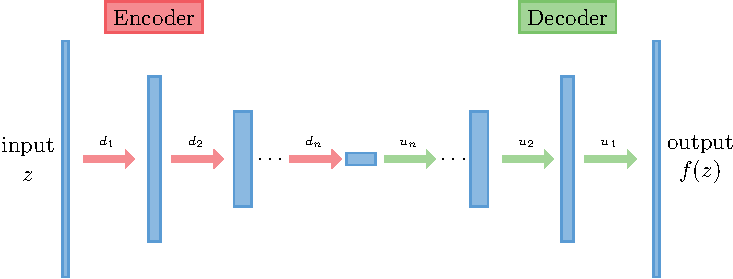
\includegraphics[width=\textwidth]{../../paper/figs/encoder_decoder.pdf}%
  \end{figure}
}

\frame{
  \frametitle{Convolutional neural network uses an encoder-decoder structure.}
  \begin{figure}[!tbp]%
    \centering%
    \begin{subfigure}[b]{0.33\textwidth}%
      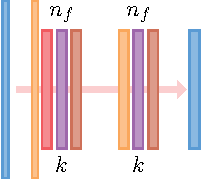
\includegraphics[width=0.92\textwidth]{../../paper/figs/downsample.pdf}%
    \end{subfigure}%
    \hfill%
    \begin{subfigure}[b]{0.33\textwidth}%
      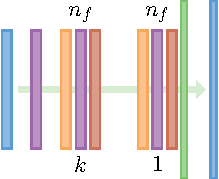
\includegraphics[width=\textwidth]{../../paper/figs/upsample.pdf}%
    \end{subfigure}%
    \hfill%
    \begin{subfigure}[b]{0.15\textwidth}%
      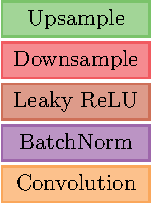
\includegraphics[width=\textwidth]{../../paper/figs/legend.pdf}%
      \vspace*{0.4cm}%
    \end{subfigure}%
  \end{figure}%
  \structure{Neural network details and implementation}\\
  \hspace*{1cm}Leaky ReLU non-linear activation functions\\
  \hspace*{1cm}Downsampling performed through striding\\
  \hspace*{1cm}Upsampling done with nearest-neighbor upsampling\\
  \hspace*{1cm}Fixed number of filters (128) in each layer, kernel size of 3\\
  \hspace*{1cm}Adam optimization, 2000 iteration (loss decrease by 1000x)\\
  \hspace*{1cm}PyTorch implementation, training on Tesla V100 GPU
}

\frame{
  \frametitle{Demonstration of the reconstruction procedure.}
  \begin{figure}[!tbp]%
    \centering%
    \begin{subfigure}[t]{0.32\textwidth}%
      
\includegraphics[width=\textwidth]{../../figs/image0.png}%
      \caption*{Original.}%
    \end{subfigure}%
    \hfill%
    \begin{subfigure}[t]{0.32\textwidth}%
      
\includegraphics[width=\textwidth]{../../figs/masked0.png}%
      \caption*{Deteriorated.}%
    \end{subfigure}%
    \hfill%
    \begin{subfigure}[t]{0.32\textwidth}%
      \includegraphics<1>[width=\textwidth]{./figs/input.png}%
      \includegraphics<2>[width=\textwidth]{./figs/iteration00000.png}%
      \includegraphics<3>[width=\textwidth]{./figs/iteration00050.png}%
      \includegraphics<4>[width=\textwidth]{./figs/iteration00100.png}%
      \includegraphics<5>[width=\textwidth]{./figs/iteration00300.png}%
      \includegraphics<6>[width=\textwidth]{./figs/iteration02000.png}%
      \only<1>{\caption*{Input.}}%
      \only<2>{\caption*{Epoch 1.}}%
      \only<3>{\caption*{Epoch 50.}}%
      \only<4>{\caption*{Epoch 100.}}%
      \only<5>{\caption*{Epoch 300.}}%
      \only<6>{\caption*{Epoch 2000.}}%
    \end{subfigure}%
  \end{figure}%
}

\frame{
  \frametitle{Gaussian process regression is used for comparisons of data recovery problems.}
  \structure{Gaussian process regression}\\
  \hspace*{1cm}commonly used for this task in geophysics (Kriging)\\
  \hspace*{1cm}kernel based probabilistic model (Bayesian method)\\
  \hspace*{1cm}computes a posterior distribution over models\\
  \hspace*{1cm}provides model uncertainty\\
  \hspace*{1cm}$\mathcal{O}(n^3)$ scaling with the number of training samples\\[0.3cm]
  \structure{For the results presented here}\\
  \hspace*{1cm}\mbox{training points from a region surrounding the deteriorated pixels}\\
  \hspace*{1cm}radial basis function GP kernel\\
  \hspace*{1cm}using GP algorithm in Scikit-Learn library\\[0.3cm]
  \structure{\mbox{Other methods (interpolation, etc) were attempted with little success}}
}

% ================================================================================
% Results

% Cylinder
\frame{
  \frametitle{Data recovery for laminar flow around a cylinder.}
  \vspace*{0.3cm}
  \structure{Simulation setup}\\
  \hspace*{1cm}laminar flow around bluff body ($Re = 200$)\\
  \hspace*{1cm}Nalu-Wind, a low Mach Navier-Stokes solver using Trilinos
  \hspace*{1cm}$t=234\unit{s}$ snapshot for data recovery (fully developed flow)\\[0.2cm]
  \structure{Recovery study}\\
  \hspace*{1cm}square masks located at 40 random downstream locations\\
  \hspace*{1cm}various mask sizes, $L_m \in [0.5D, 5D]$
  \begin{figure}[!tbp]%
    \centering%
    \includegraphics<1>[width=0.8\textwidth]{../../paper/figs/cyl_umag0.png}%
    \includegraphics<2>[width=0.8\textwidth]{../../paper/figs/cyl_umag0_masked.png}%
  \end{figure}%
}

\frame{
  \frametitle{Results indicate that the CNN recovers the flow accurately for modest mask sizes ($L_m=2D$).}
  \vspace*{0.3cm}
  \begin{figure}[!tbp]%
    \centering%
    \begin{subfigure}[t]{0.45\textwidth}%
      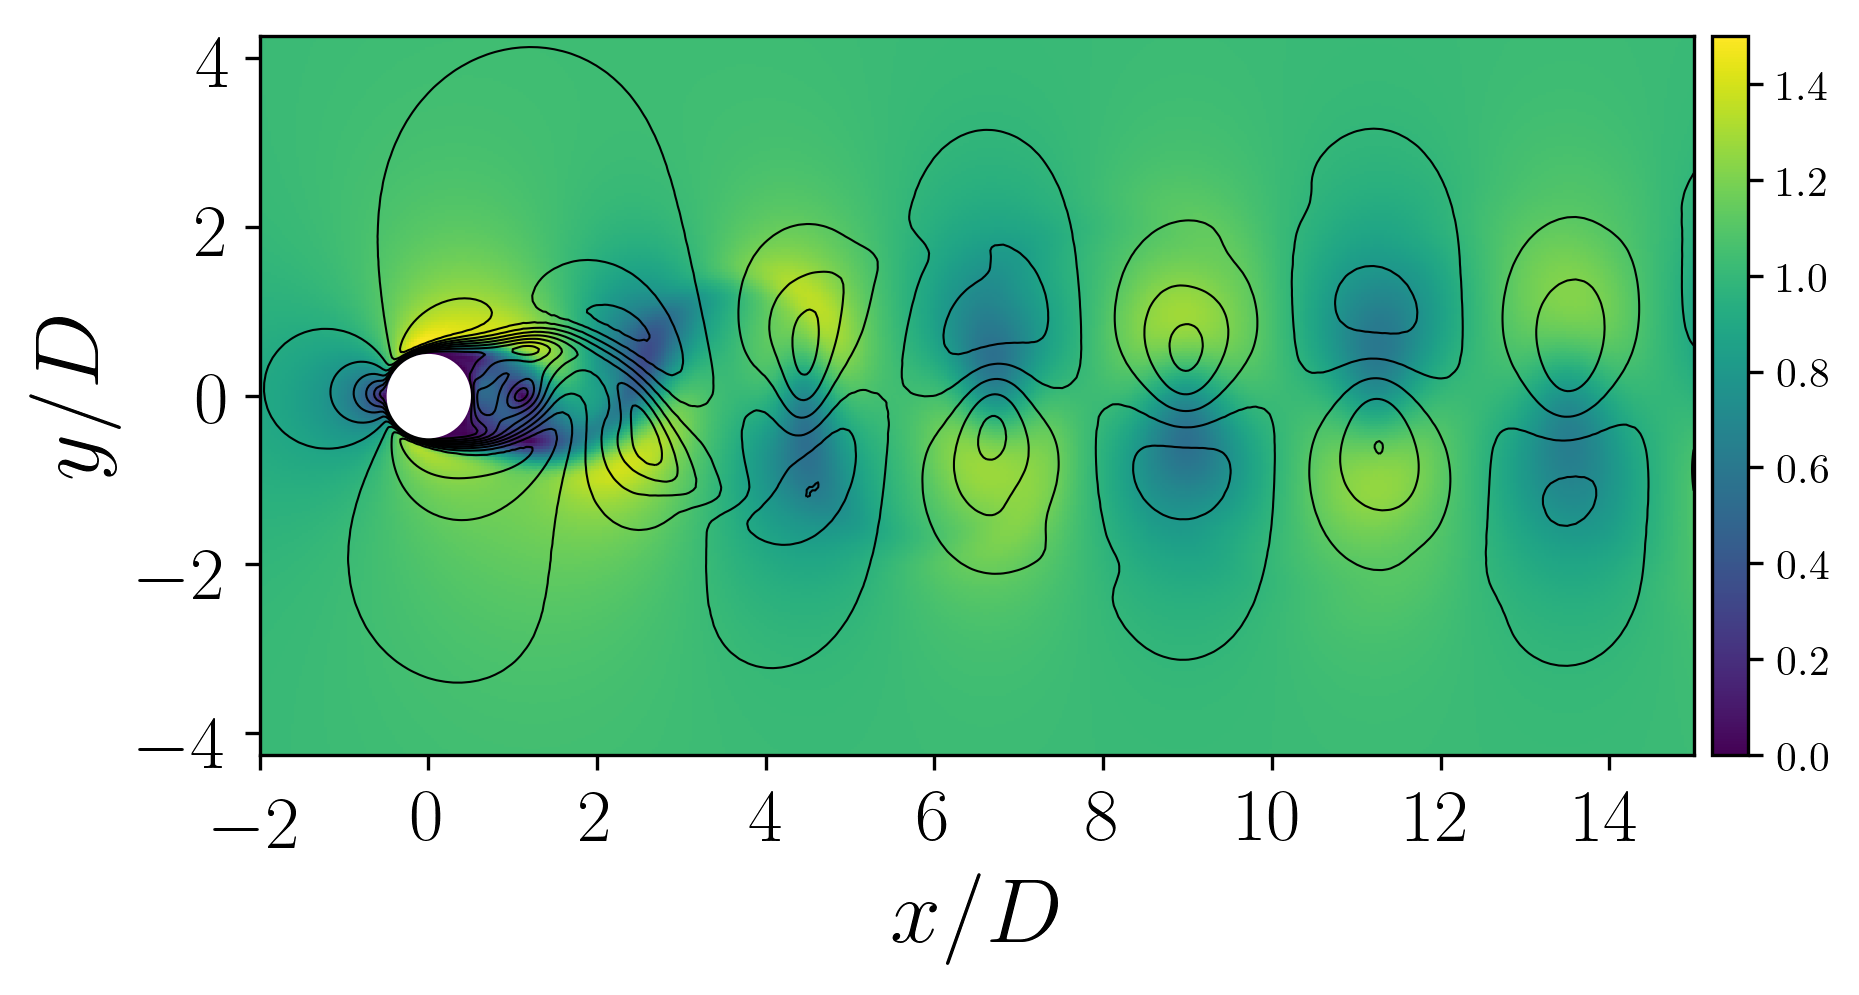
\includegraphics[width=\textwidth]{../../paper/figs/cyl_umag0.png}%
      \caption*{Original data.}\label{fig:cyl_umag0}%
    \end{subfigure}%
    \hfill%
    \begin{subfigure}[t]{0.45\textwidth}%
      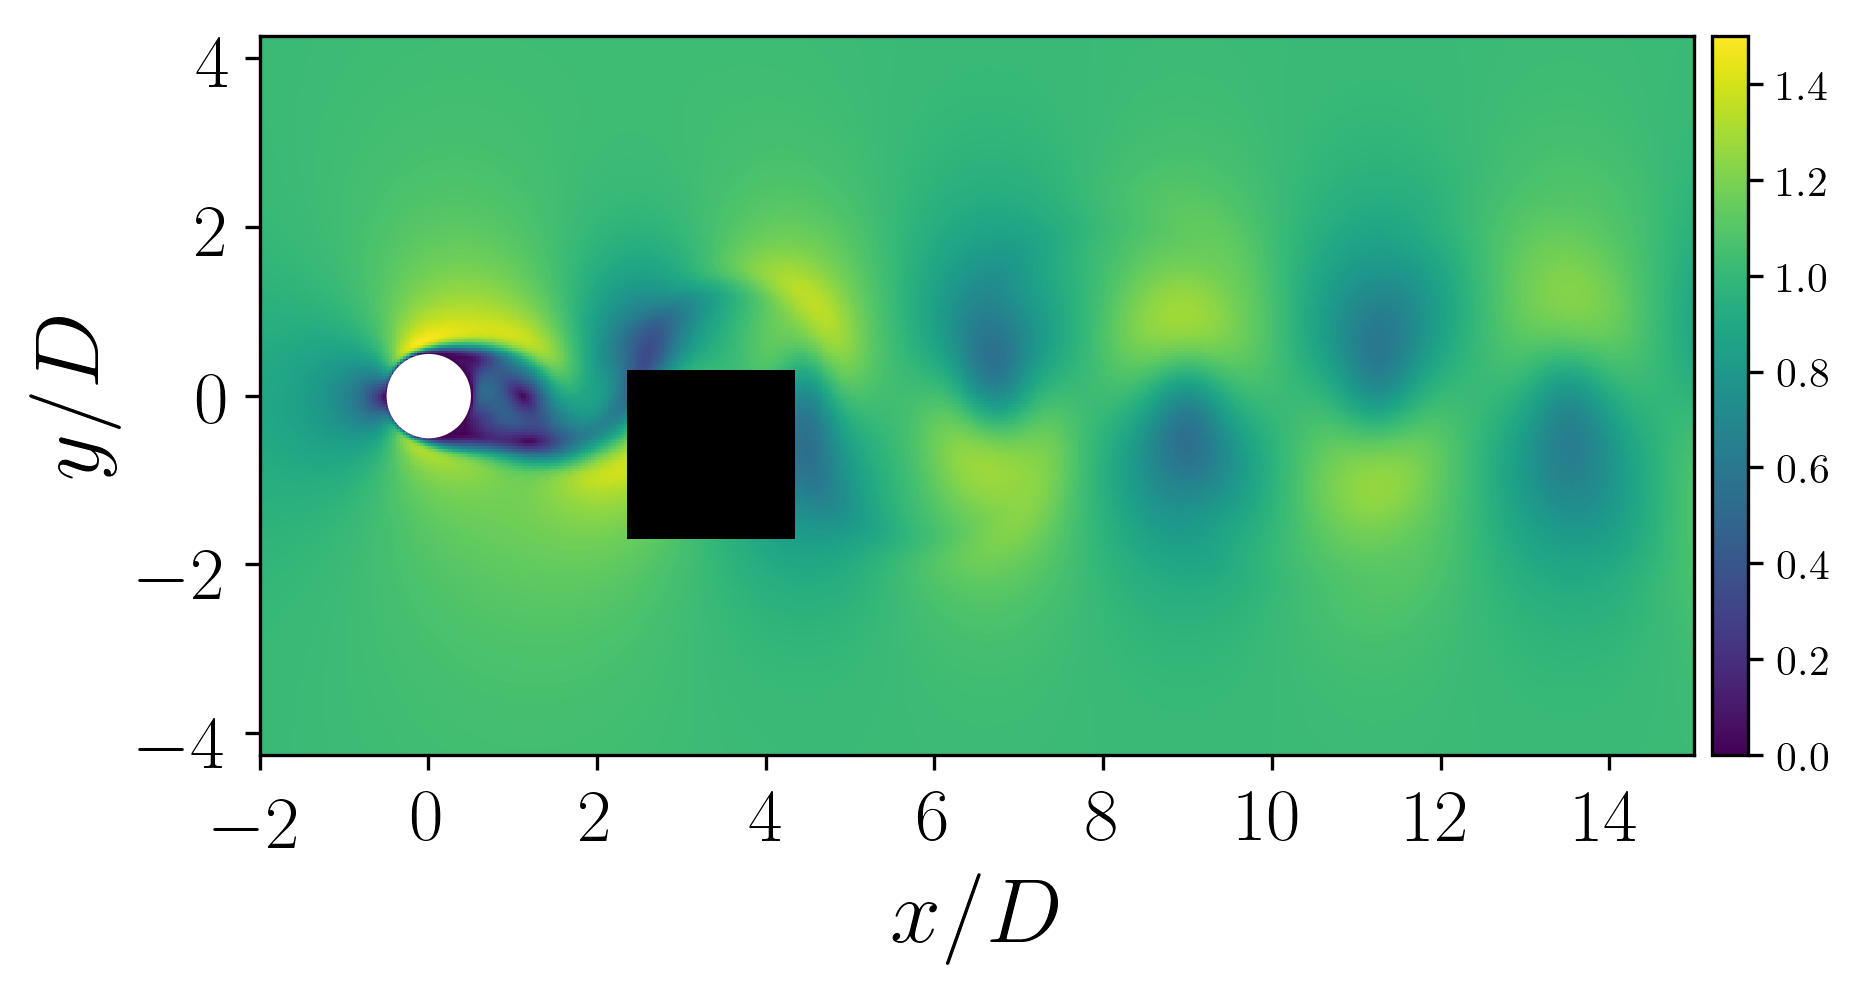
\includegraphics[width=\textwidth]{../../paper/figs/cyl_umag0_masked.png}%
      \caption*{Deteriorated data.}\label{fig:cyl_umag0_masked}%
    \end{subfigure}\\%
    \begin{subfigure}[t]{0.45\textwidth}%
      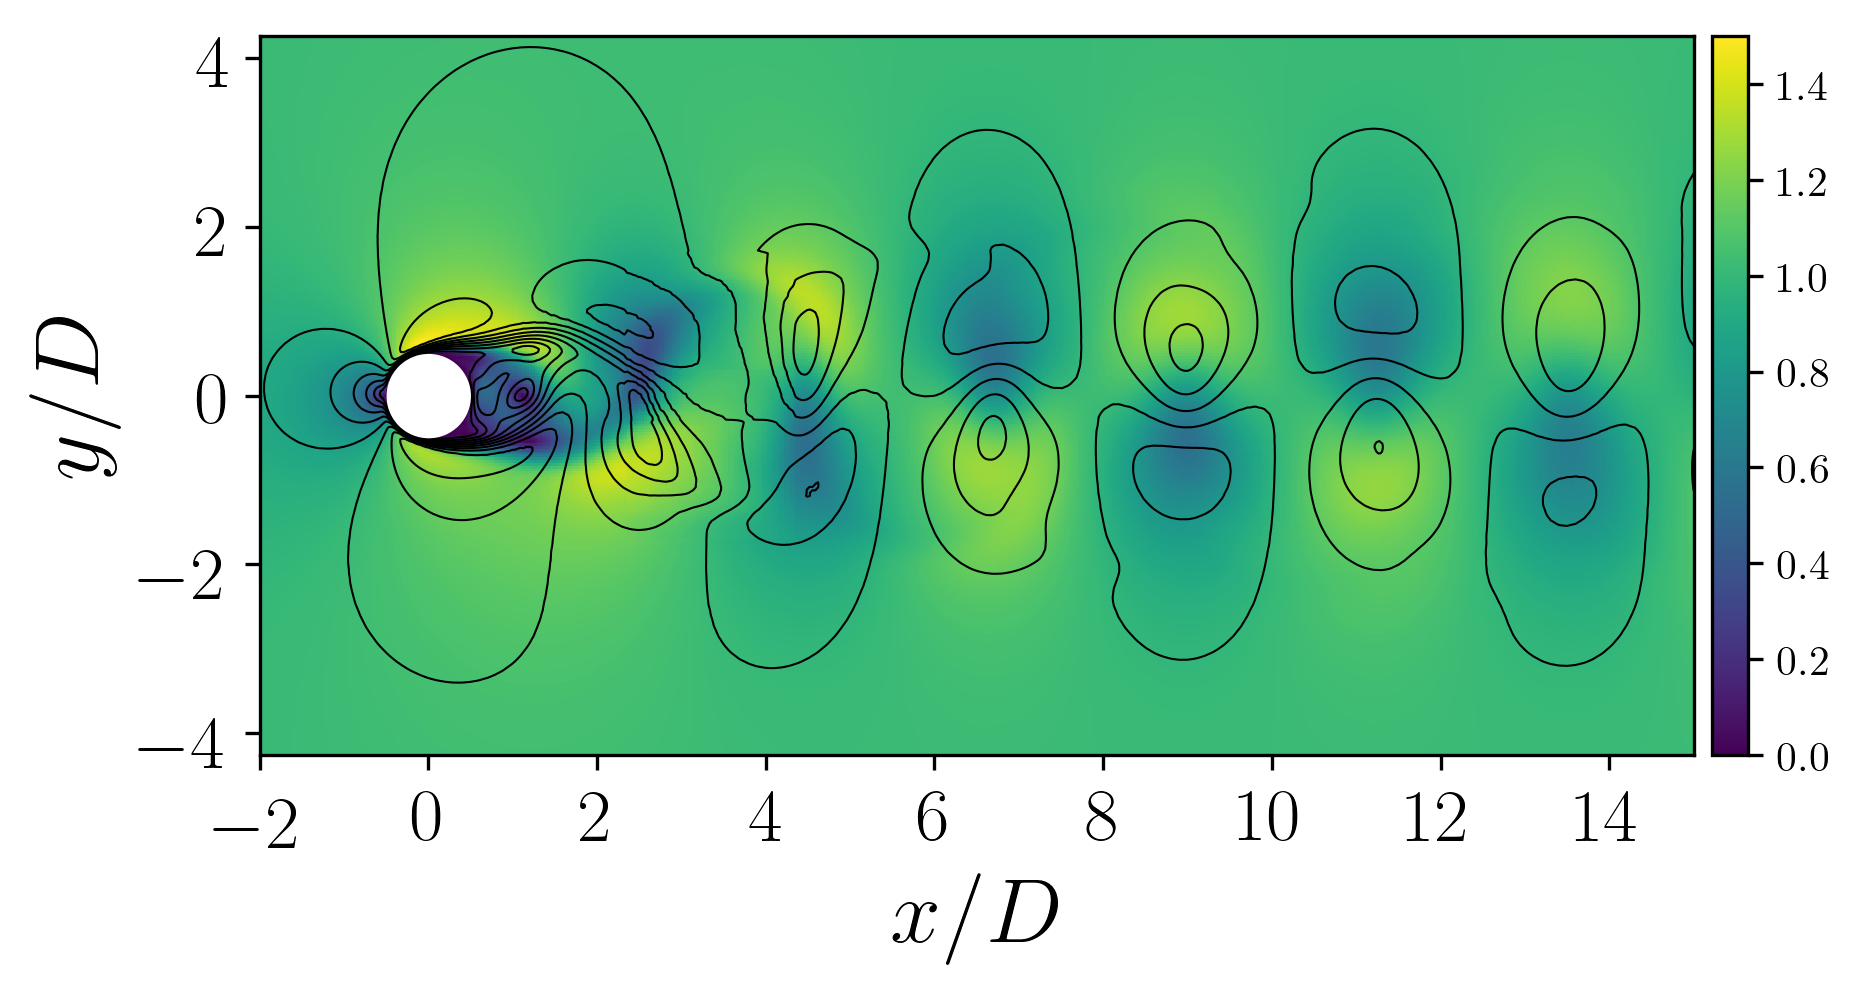
\includegraphics[width=\textwidth]{../../paper/figs/cyl_umagr.png}%
      \caption*{CNN.}\label{fig:cyl_umagr}%
    \end{subfigure}%
    \hfill%
    \begin{subfigure}[t]{0.45\textwidth}%
      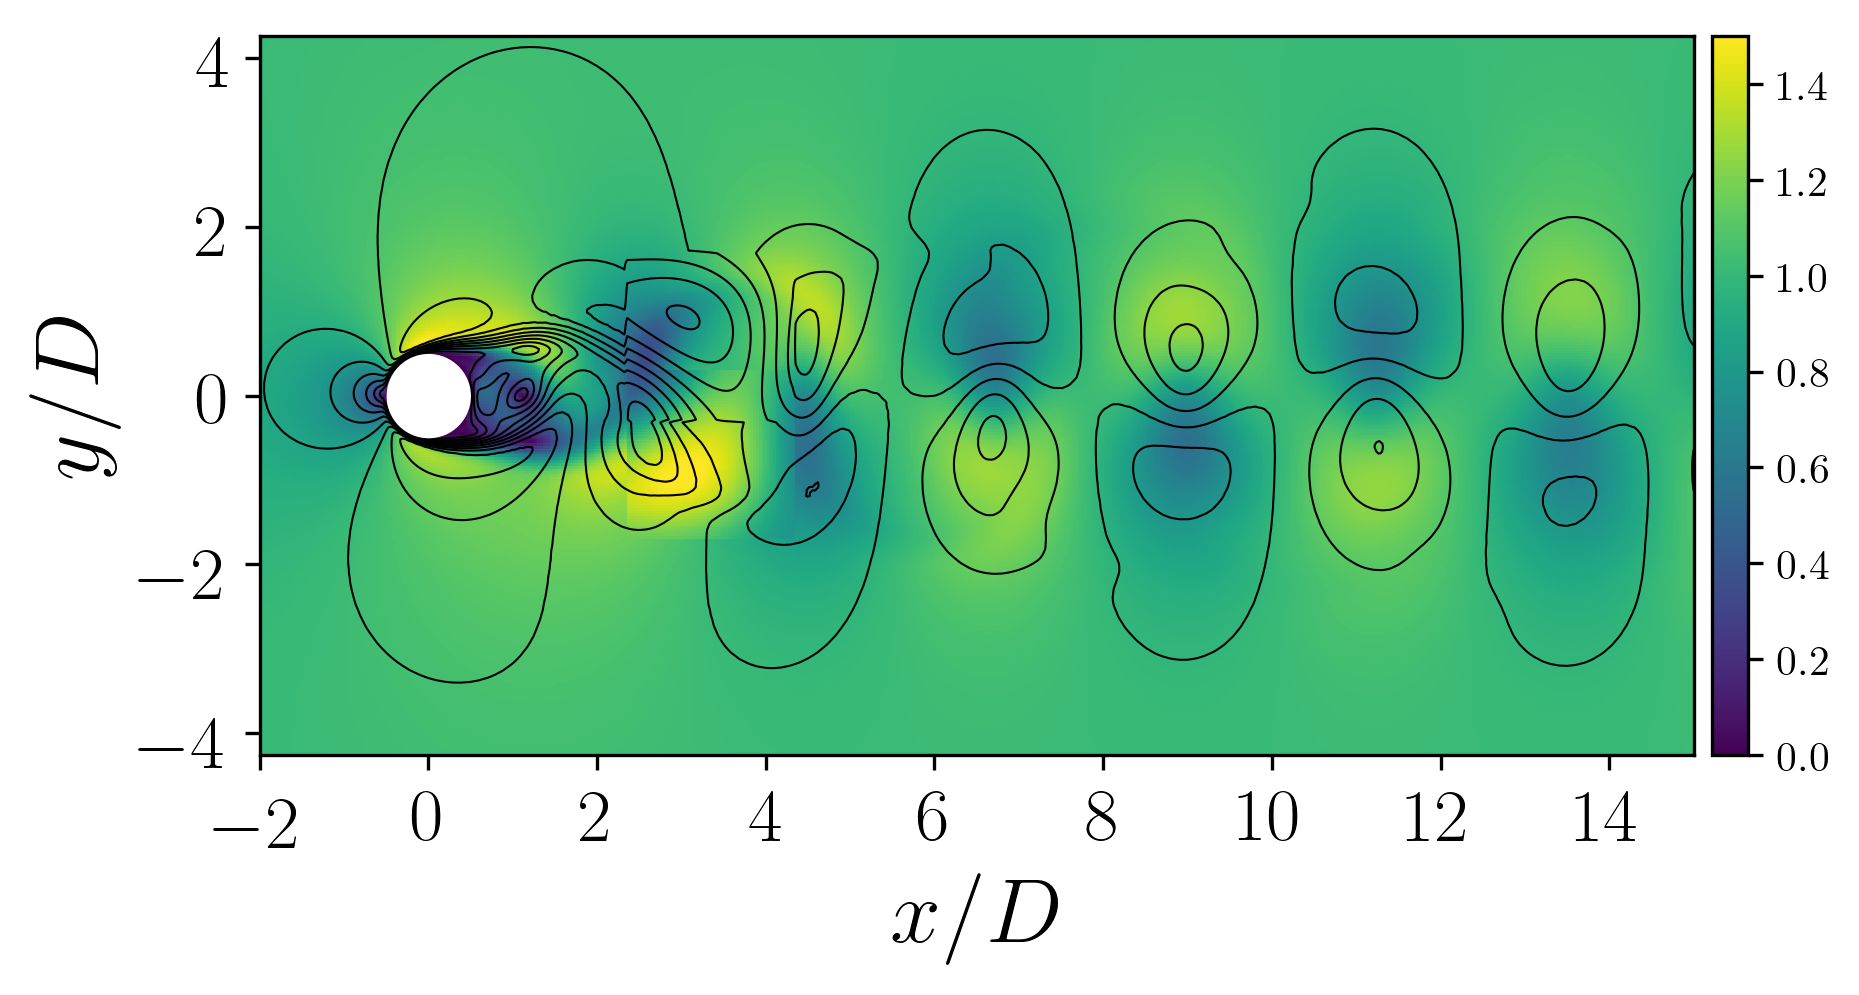
\includegraphics[width=\textwidth]{../../paper/figs/cyl_umagi.png}%
      \caption*{GPR.}\label{fig:cyl_umagi}%
    \end{subfigure}%
  \end{figure}%
}

\frame{
  \frametitle{CNN does not significantly outperform GPR over a range of mask sizes for this laminar flow.}
  \vspace*{0.3cm}
  \begin{align*}
    L_2(u) = \sqrt{\frac{1}{N} \sum_i (u(i) - u_r(i))^2}
  \end{align*}
  \begin{figure}[!tbp]%
    \centering%
    \begin{subfigure}[t]{0.48\textwidth}%
      \begin{tikzpicture}
        \node[anchor=south west,inner sep=0] (image) at (0,0) {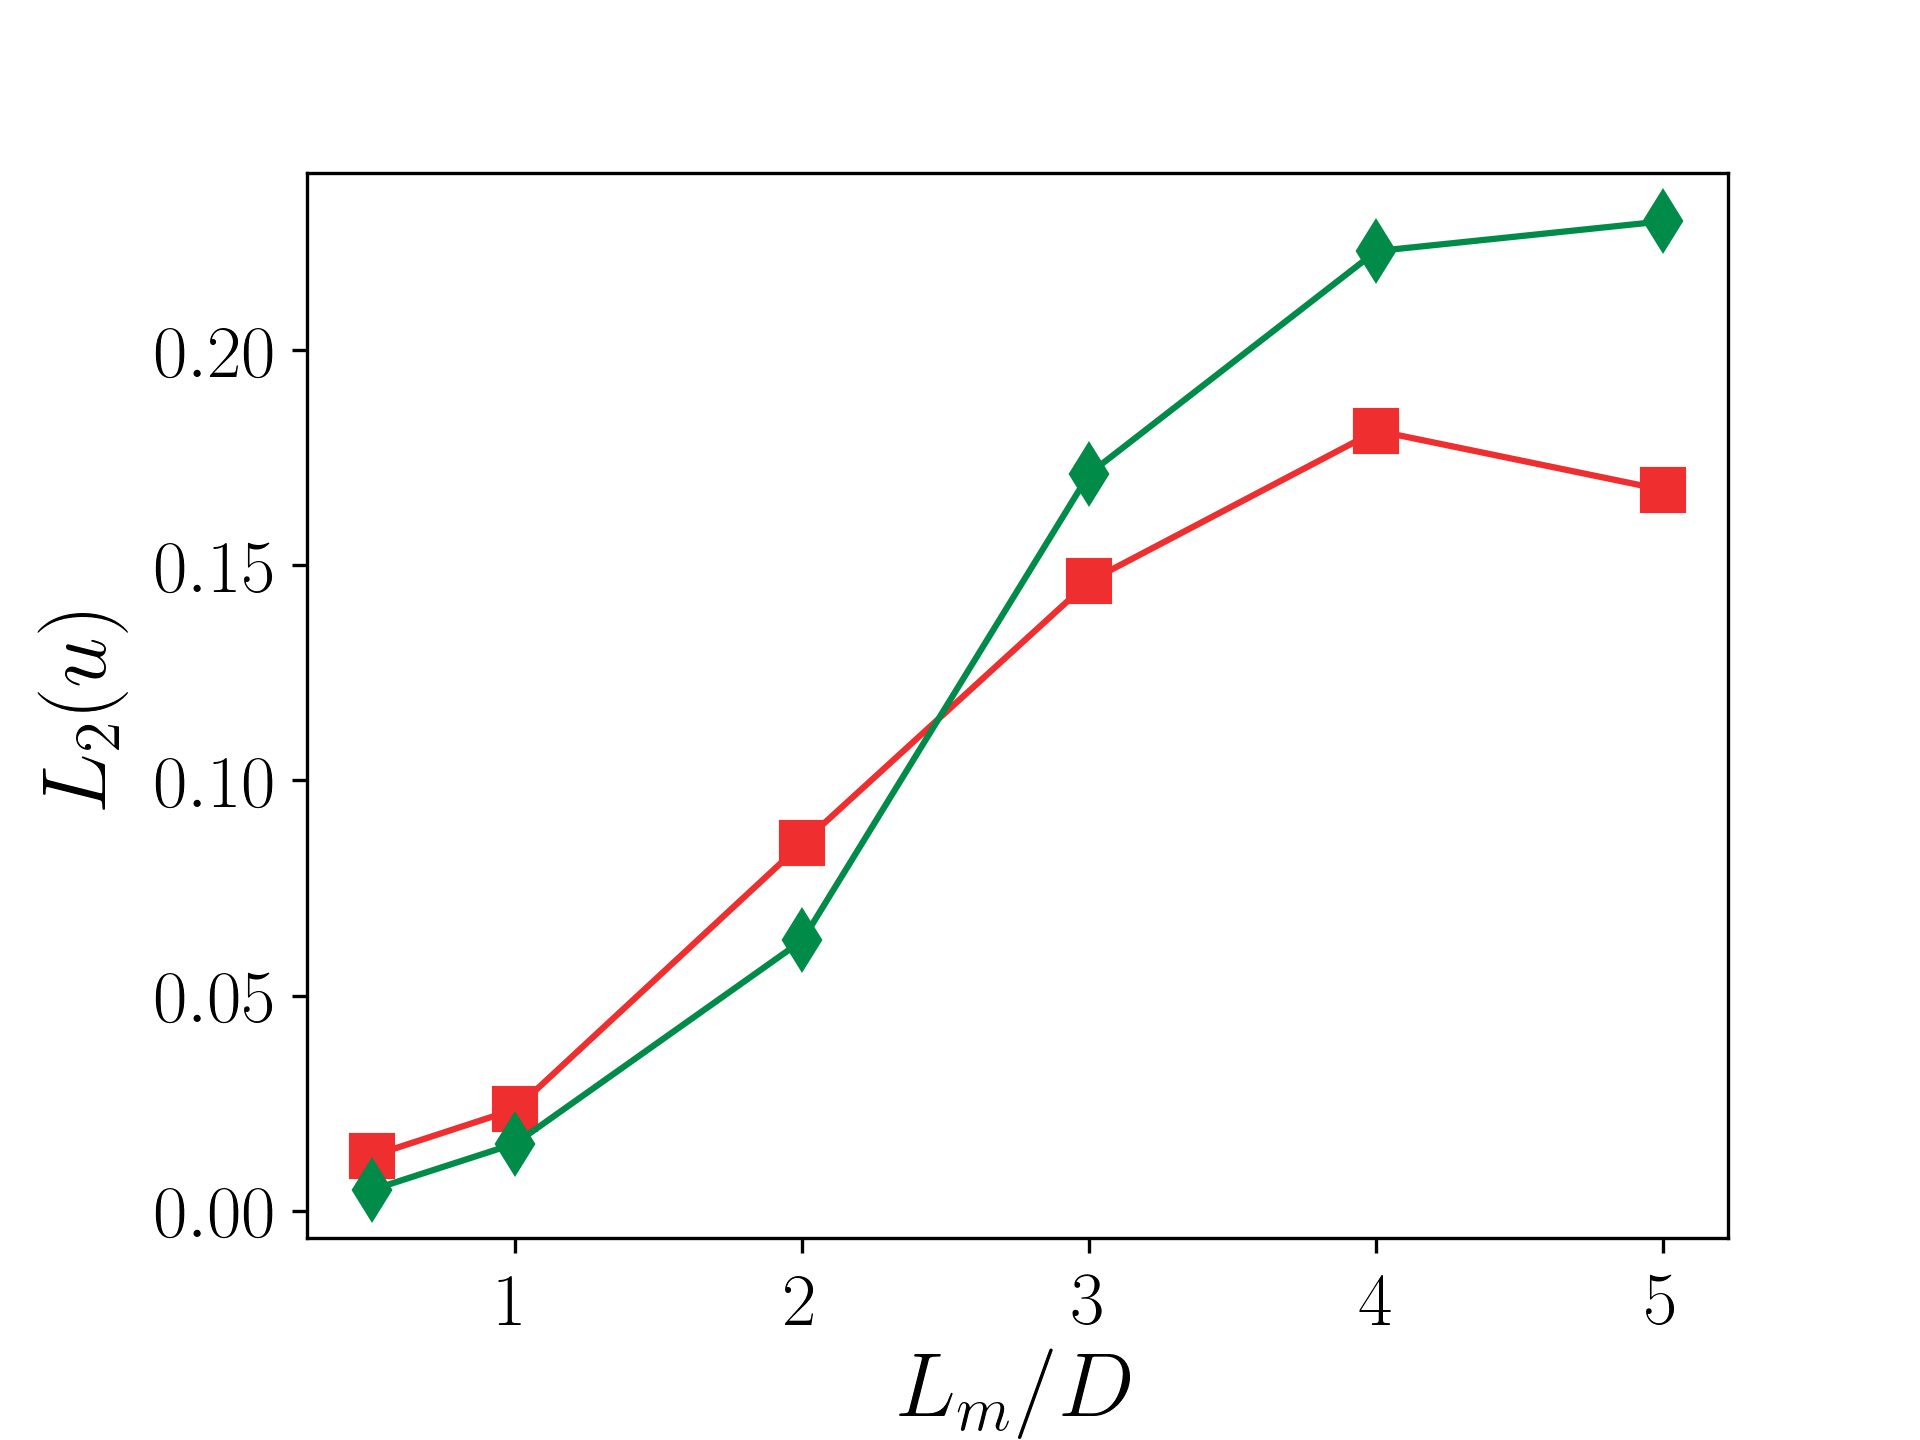
\includegraphics[width=\textwidth]{../../paper/figs/cyl_error_u.png}};
        \begin{scope}[x={(image.south east)},y={(image.north west)}]
          \draw (0.8, 0.6) node[font=\scriptsize] {\textcolor{c1brt}{CNN}};
          \draw (0.8, 0.78) node[font=\scriptsize] {\textcolor{c2brt}{GPR}};
        \end{scope}
      \end{tikzpicture}
      \caption*{$x$-direction velocity.}\label{fig:cyl_error_u}%
    \end{subfigure}%
    \hfill%
    \begin{subfigure}[t]{0.48\textwidth}%
      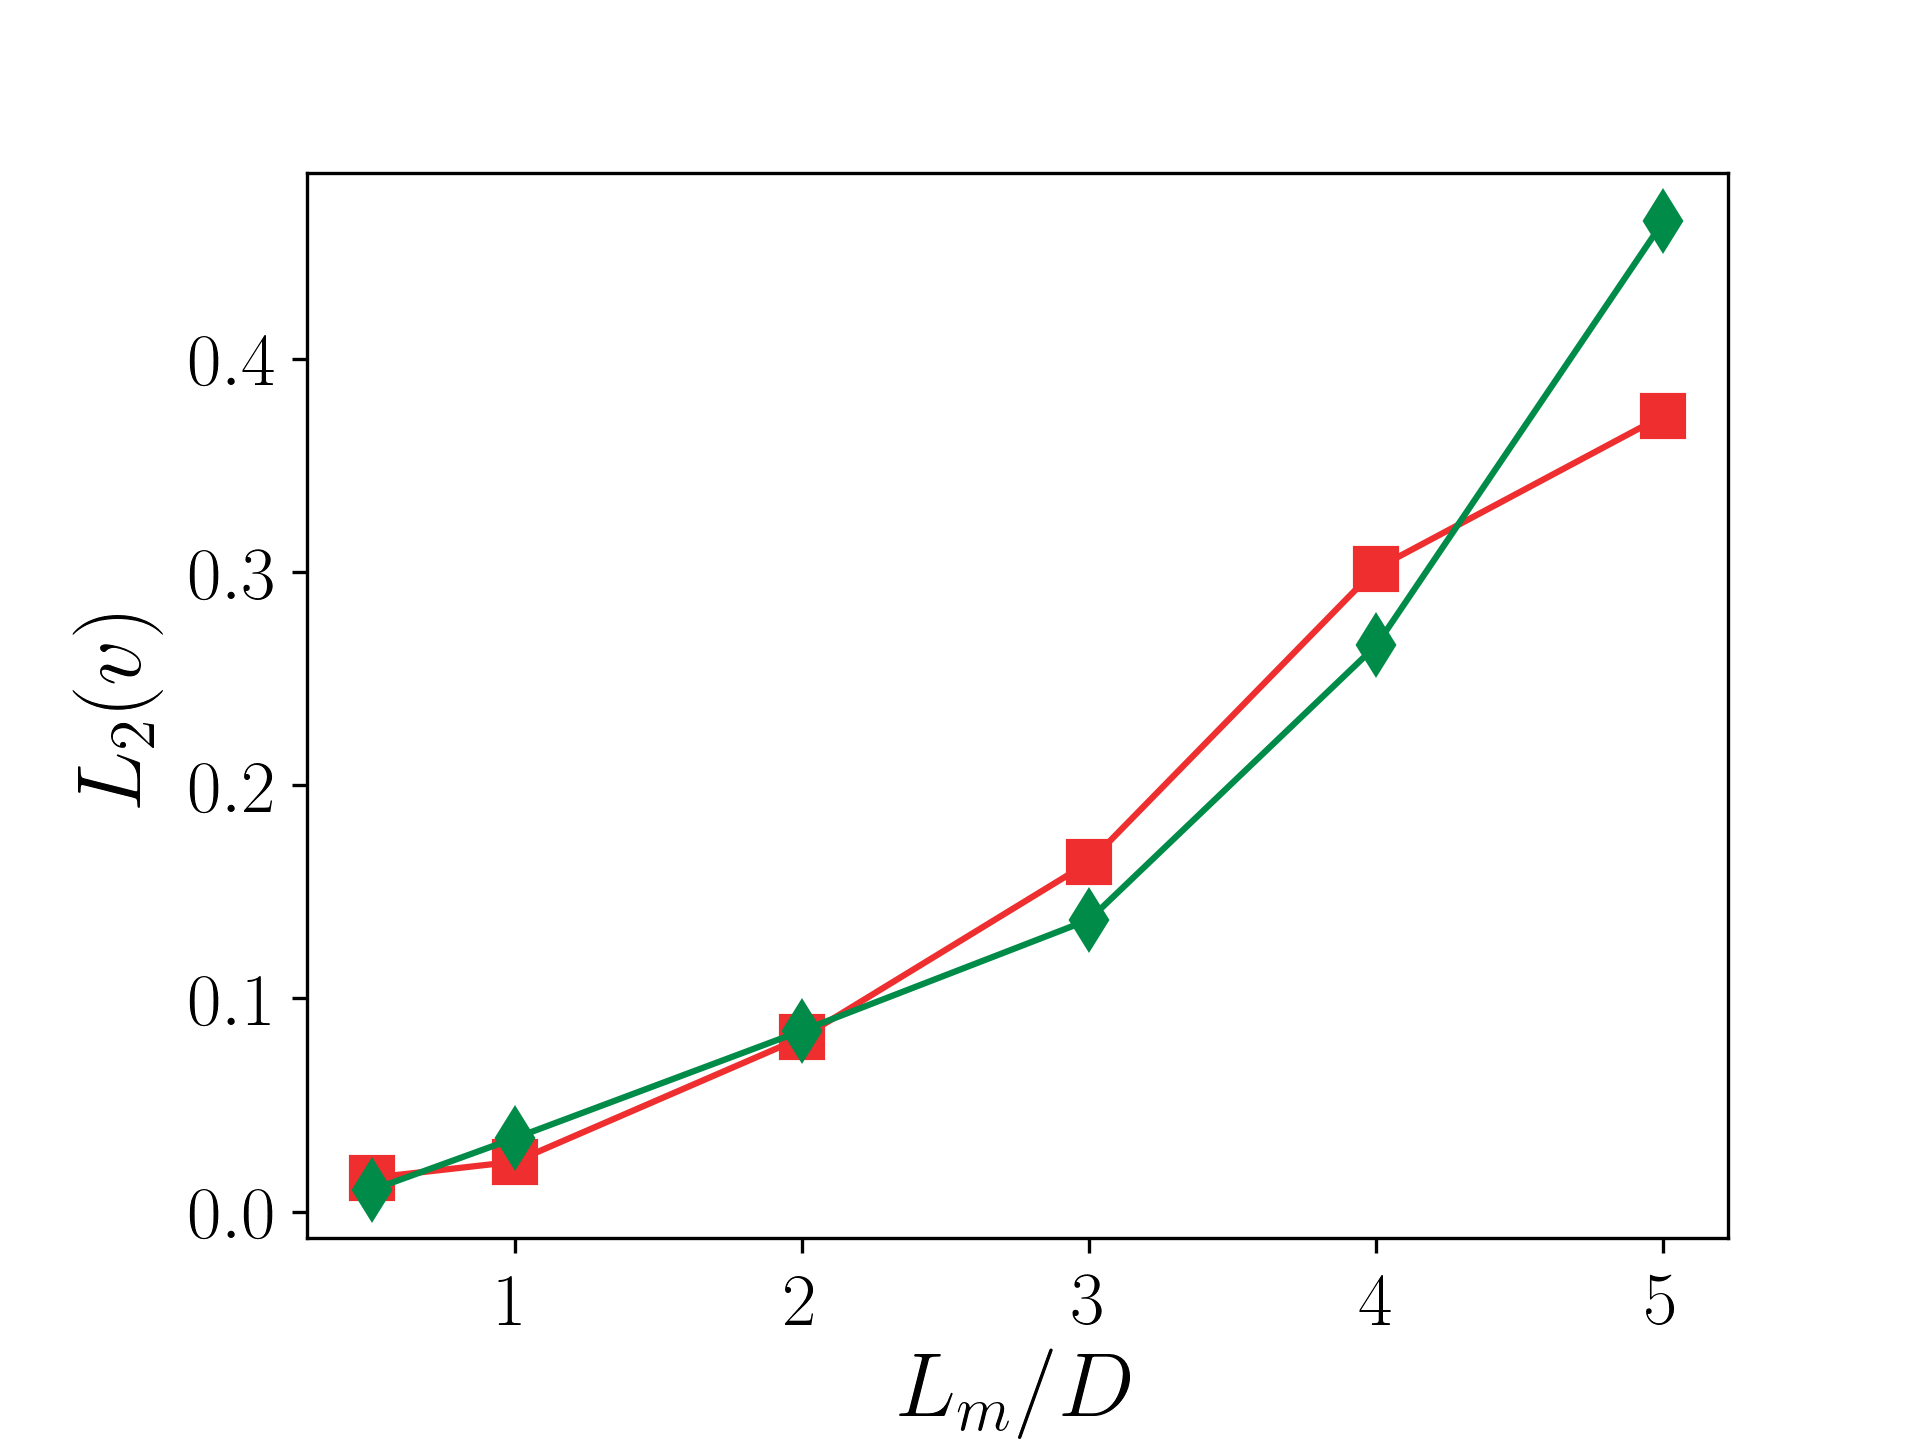
\includegraphics[width=\textwidth]{../../paper/figs/cyl_error_v.png}%
      \caption*{$y$-direction velocity.}\label{fig:cyl_error_v}%
    \end{subfigure}%
  \end{figure}%
}

% HIT
\frame{
  \frametitle{Data recovery for homogeneous isotropic turbulence.}
  \vspace*{0.3cm}
  \structure{Simulation setup}\\
  \hspace*{1cm}homogeneous isotropic turbulence ($Re_\lambda = 133$)\\
  \hspace*{1cm}PeleC, a compressible Navier-Stokes solver using AMReX\\[0.2cm]
  \structure{Recovery study}\\
  \hspace*{1cm}total percentage of missing data, $f \in [6.25\%, 25\%]$\\
  \hspace*{1cm}mask sizes: $L_m \in [0.03125L, 0.5L]$ or $[0.74\lambda, 11.87\lambda]$\\[0.1cm]
  \begin{figure}[!tbp]%
    \centering%
    \includegraphics<1>[width=0.5\textwidth]{../../paper/figs/umag0.png}%
    \includegraphics<2>[width=0.5\textwidth]{../../paper/figs/umag0_masked.png}%
  \end{figure}%
  \begin{textblock*}{2.cm}(0.75\paperwidth,.7\paperheight)%
    \only<2>{$f=25\%$\\
      $L_m = 1.5\lambda$}
  \end{textblock*}%
}

\frame{
  \frametitle{Example of data recovery for homogeneous isotropic turbulence using deep image priors.}
  \begin{figure}[!tbp]%
    \centering%
    \begin{subfigure}[t]{0.32\textwidth}%
      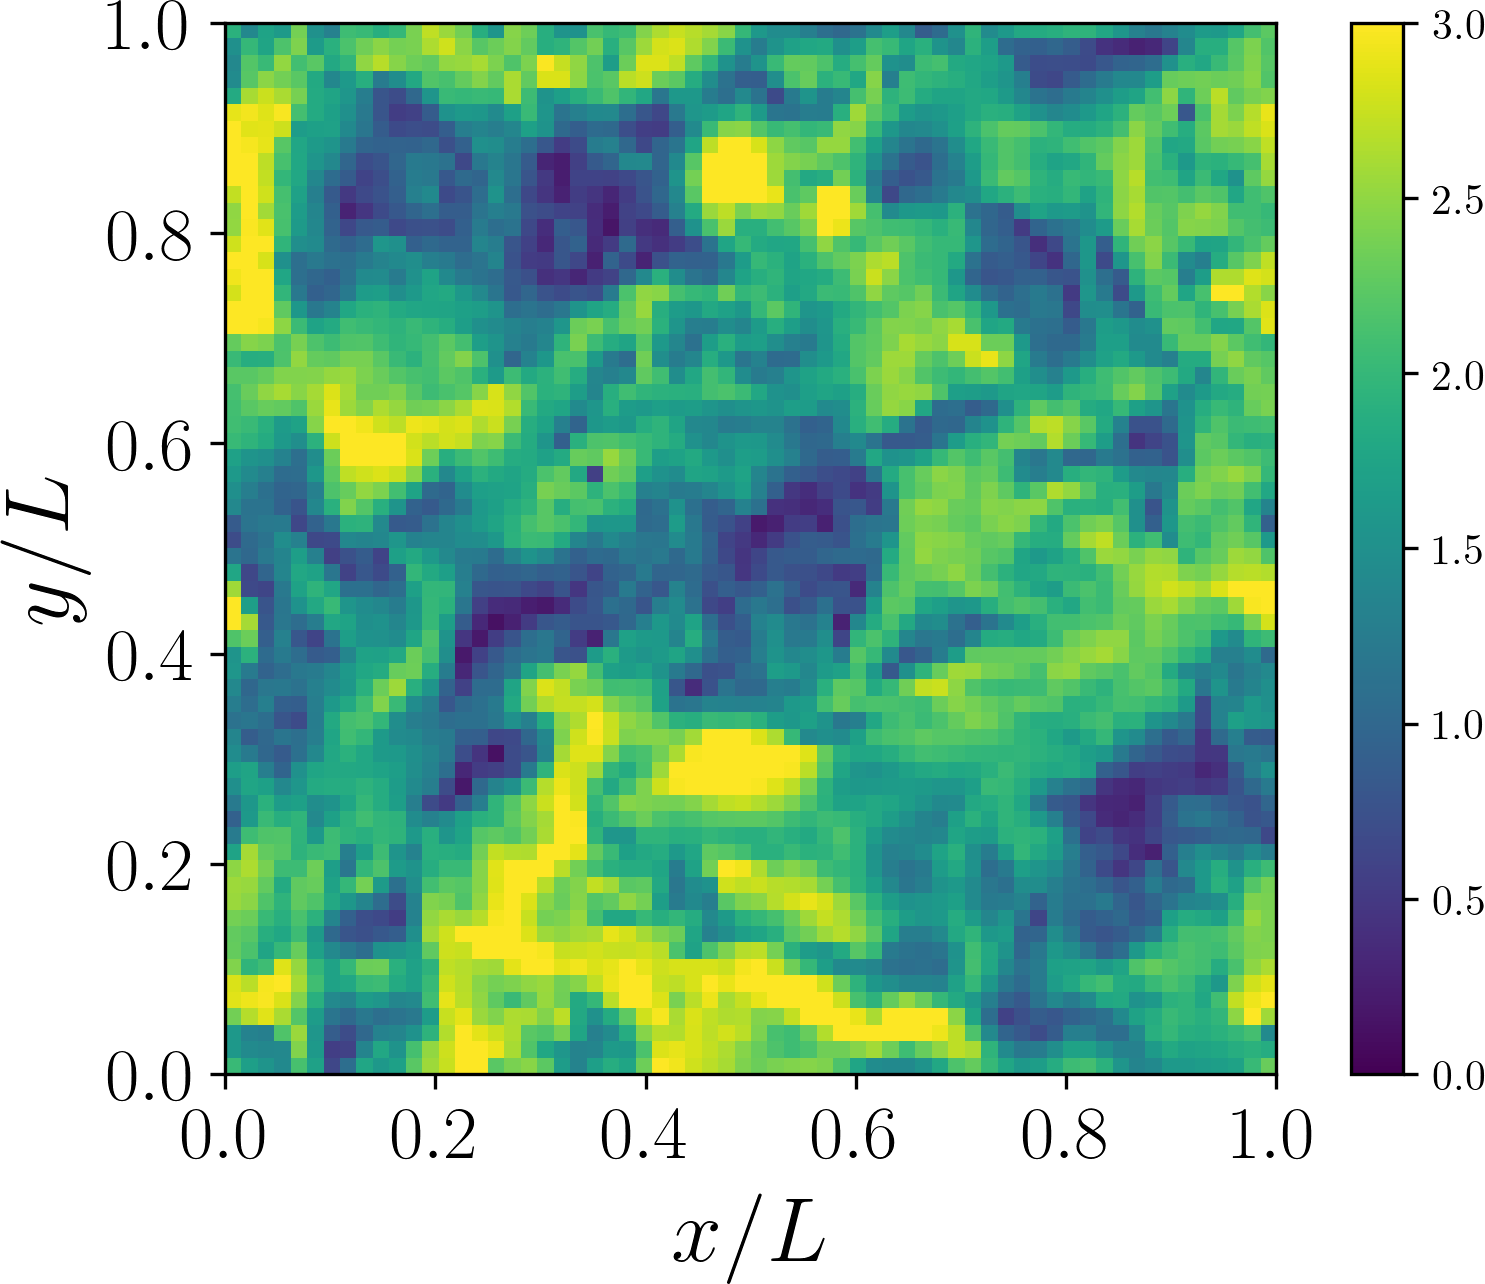
\includegraphics[width=\textwidth]{../../paper/figs/umag0.png}%
      \caption*{Original.}\label{fig:original}%
    \end{subfigure}%
    \hfill%
    \begin{subfigure}[t]{0.32\textwidth}%
      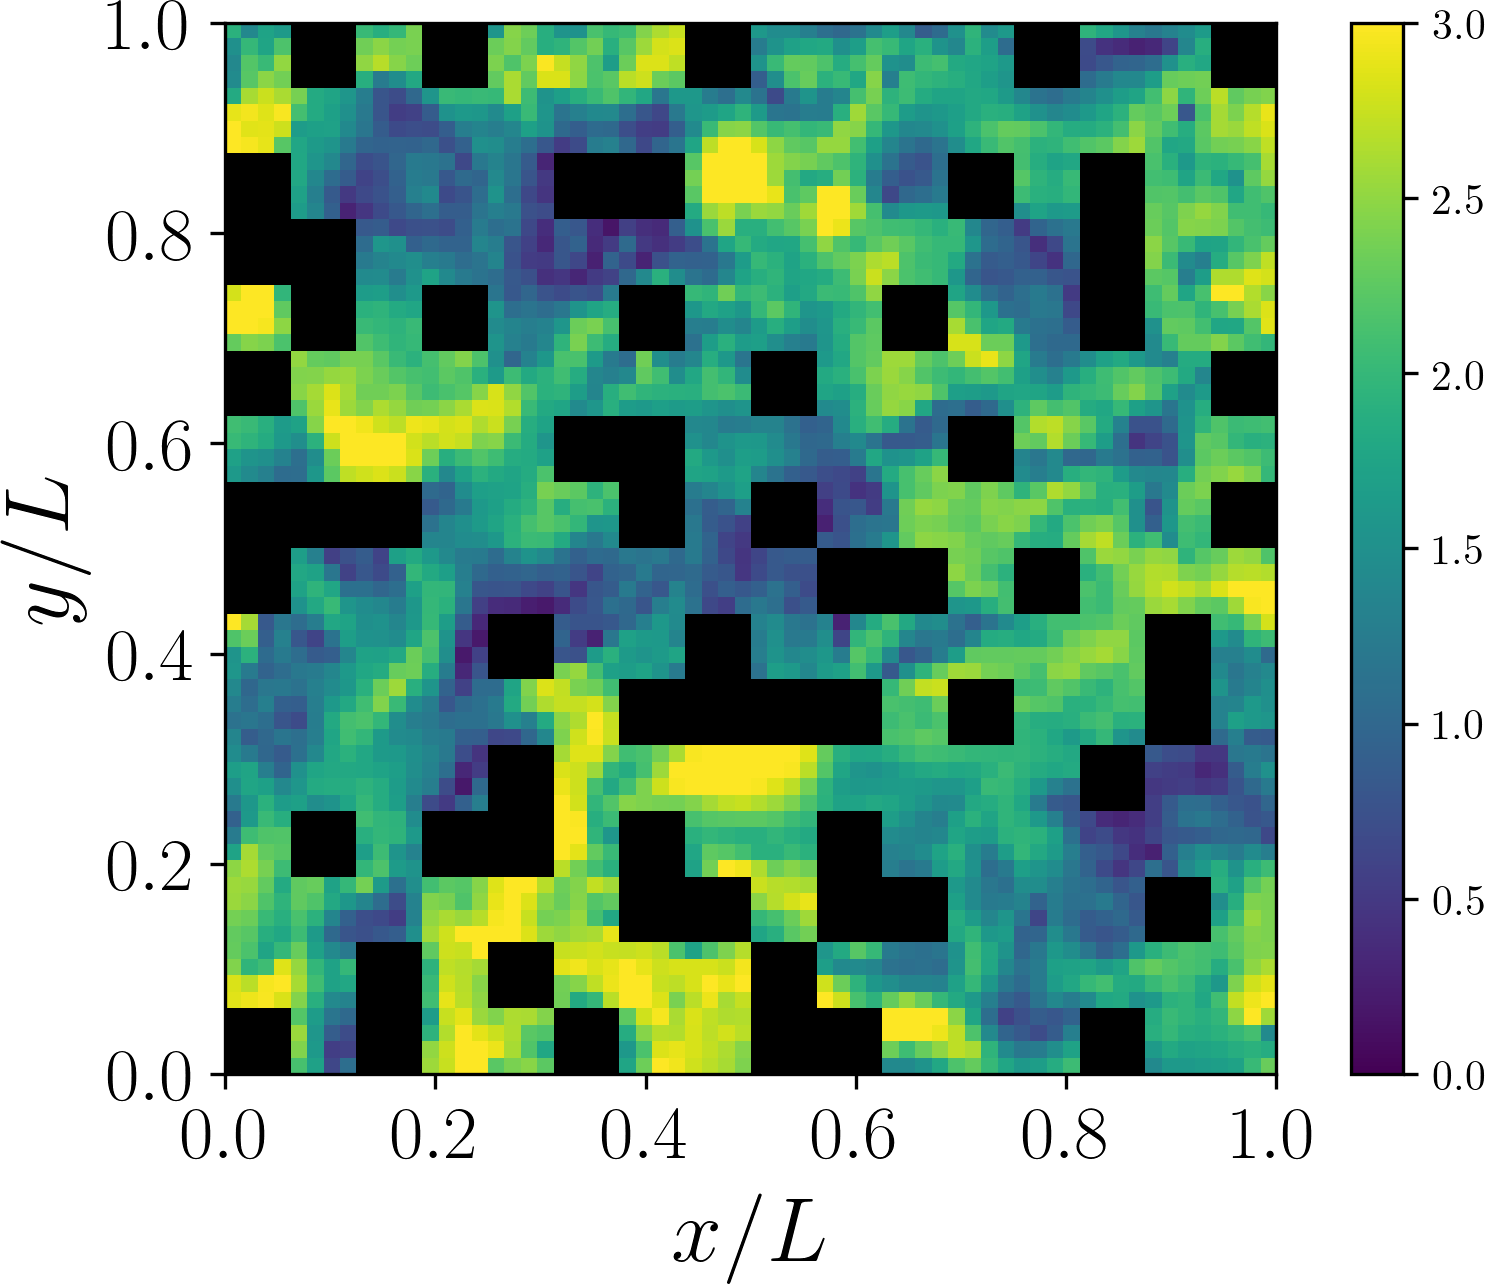
\includegraphics[width=\textwidth]{../../paper/figs/umag0_masked.png}%
      \caption*{Deteriorated.}\label{fig:masked}%
    \end{subfigure}%
    \hfill%
    \begin{subfigure}[t]{0.32\textwidth}%
      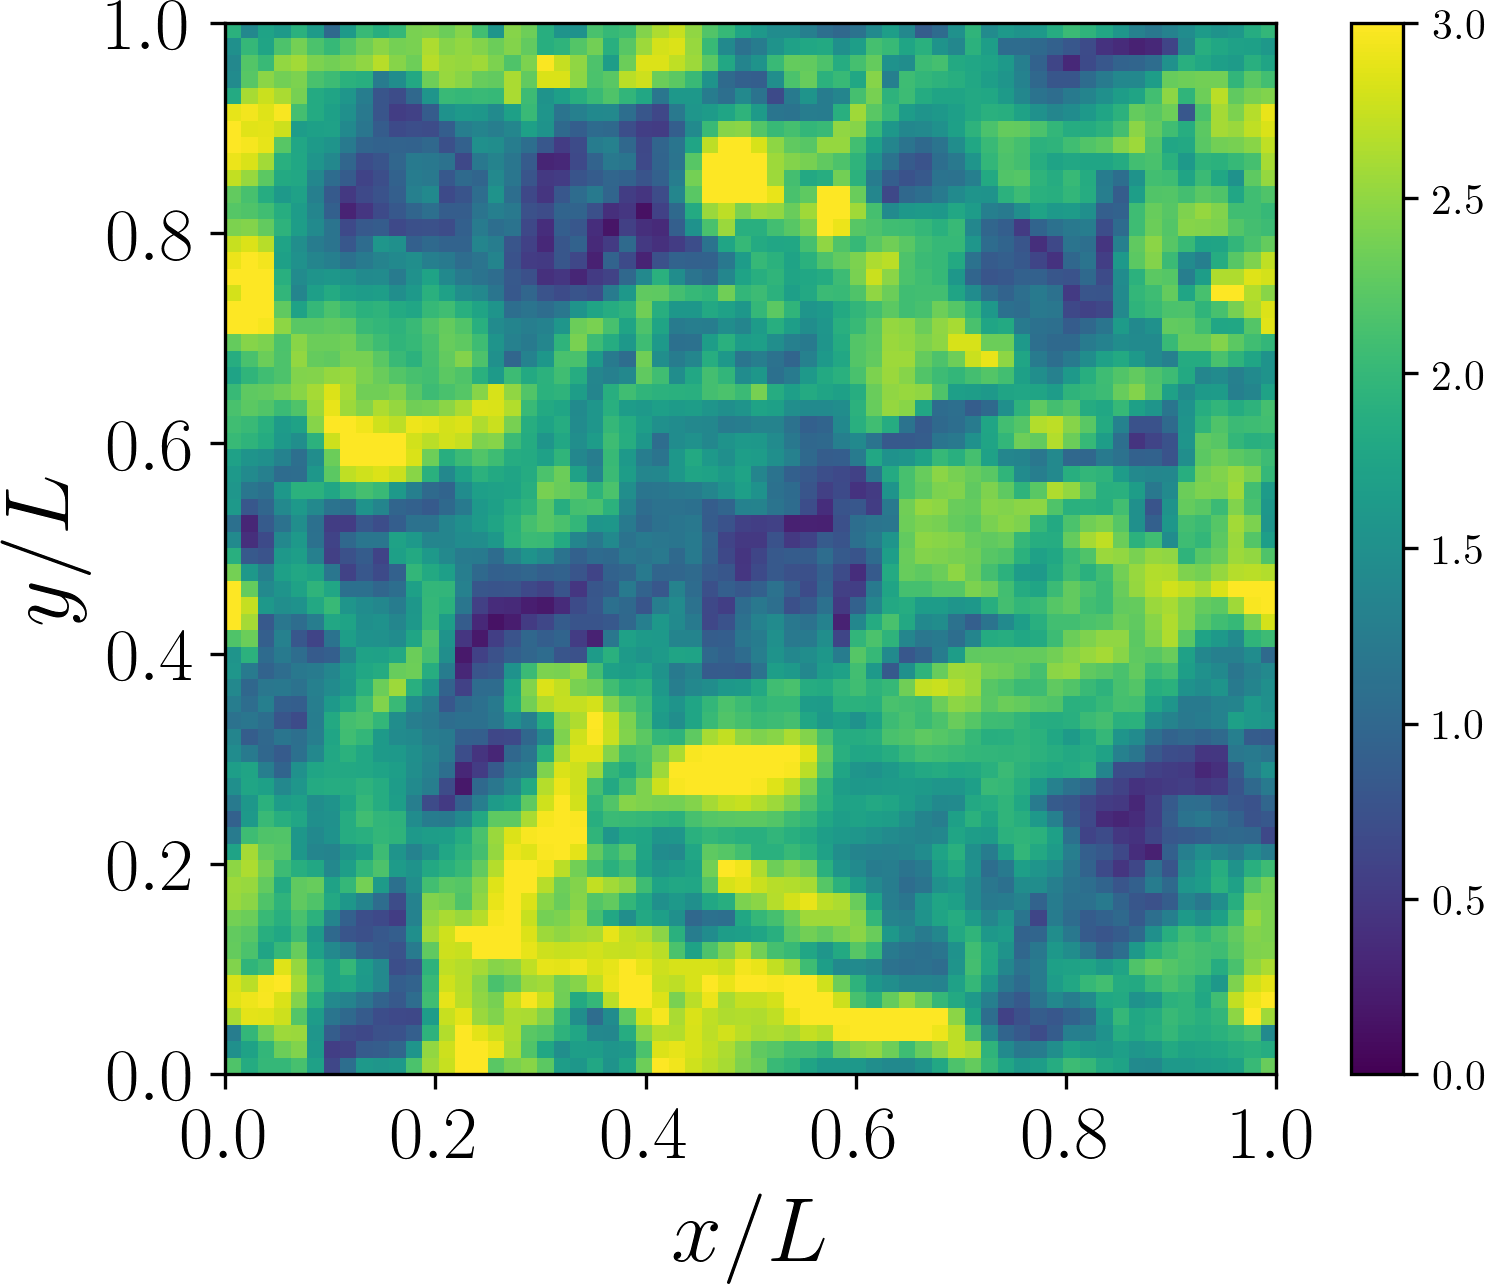
\includegraphics[width=\textwidth]{../../paper/figs/umagr.png}%
      \caption*{Recovered.}\label{fig:result}%
    \end{subfigure}%
  \end{figure}%
  We performed 1300 data recovery tasks using a variety of masks.
}

\frame{
  \frametitle{Turbulent energy spectra are used to quantify the reconstruction. CNN recovers the correct energy spectra.} 
  \begin{figure}[!tbp]%
    \centering%
    \begin{subfigure}[t]{0.48\textwidth}%
      \begin{tikzpicture}
        \node[anchor=south west,inner sep=0] (image) at (0,0) {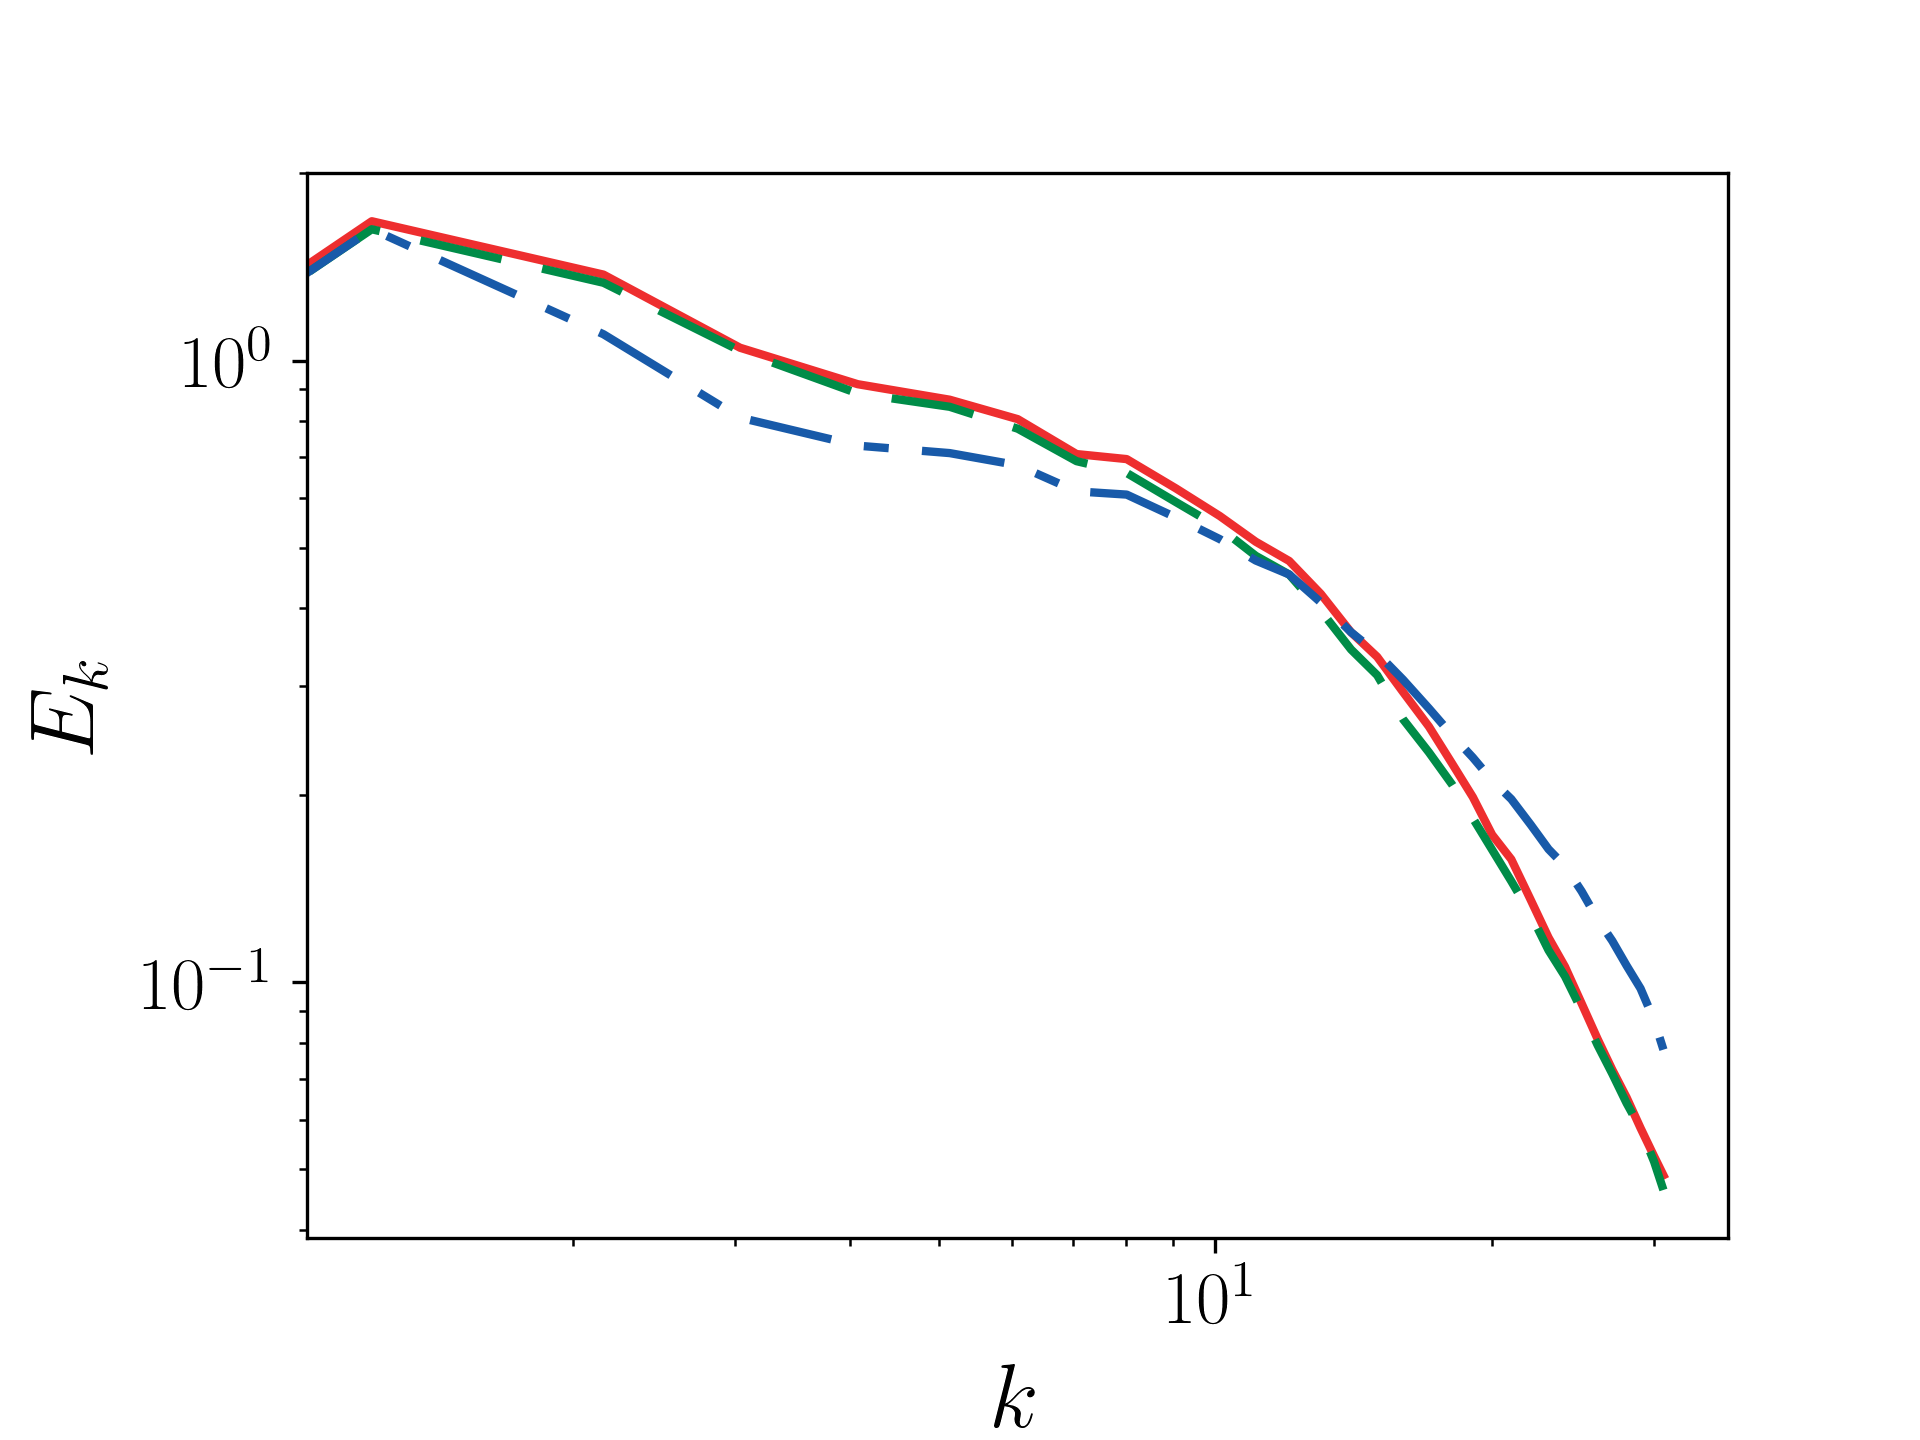
\includegraphics[width=\textwidth]{../../paper/figs/spectra.png}};
        \begin{scope}[x={(image.south east)},y={(image.north west)}]
          \draw (0.4, 0.78) node[right, font=\scriptsize] {\textcolor{c1brt}{Original} \& \textcolor{c2brt}{CNN}};
          \draw (0.4, 0.65) node[font=\scriptsize] {\textcolor{c3brt}{GPR}};
        \end{scope}
      \end{tikzpicture}
      \caption*{Average energy spectrum.}\label{fig:spectra}%
    \end{subfigure}%
    \hfill%
    \begin{subfigure}[t]{0.48\textwidth}%
      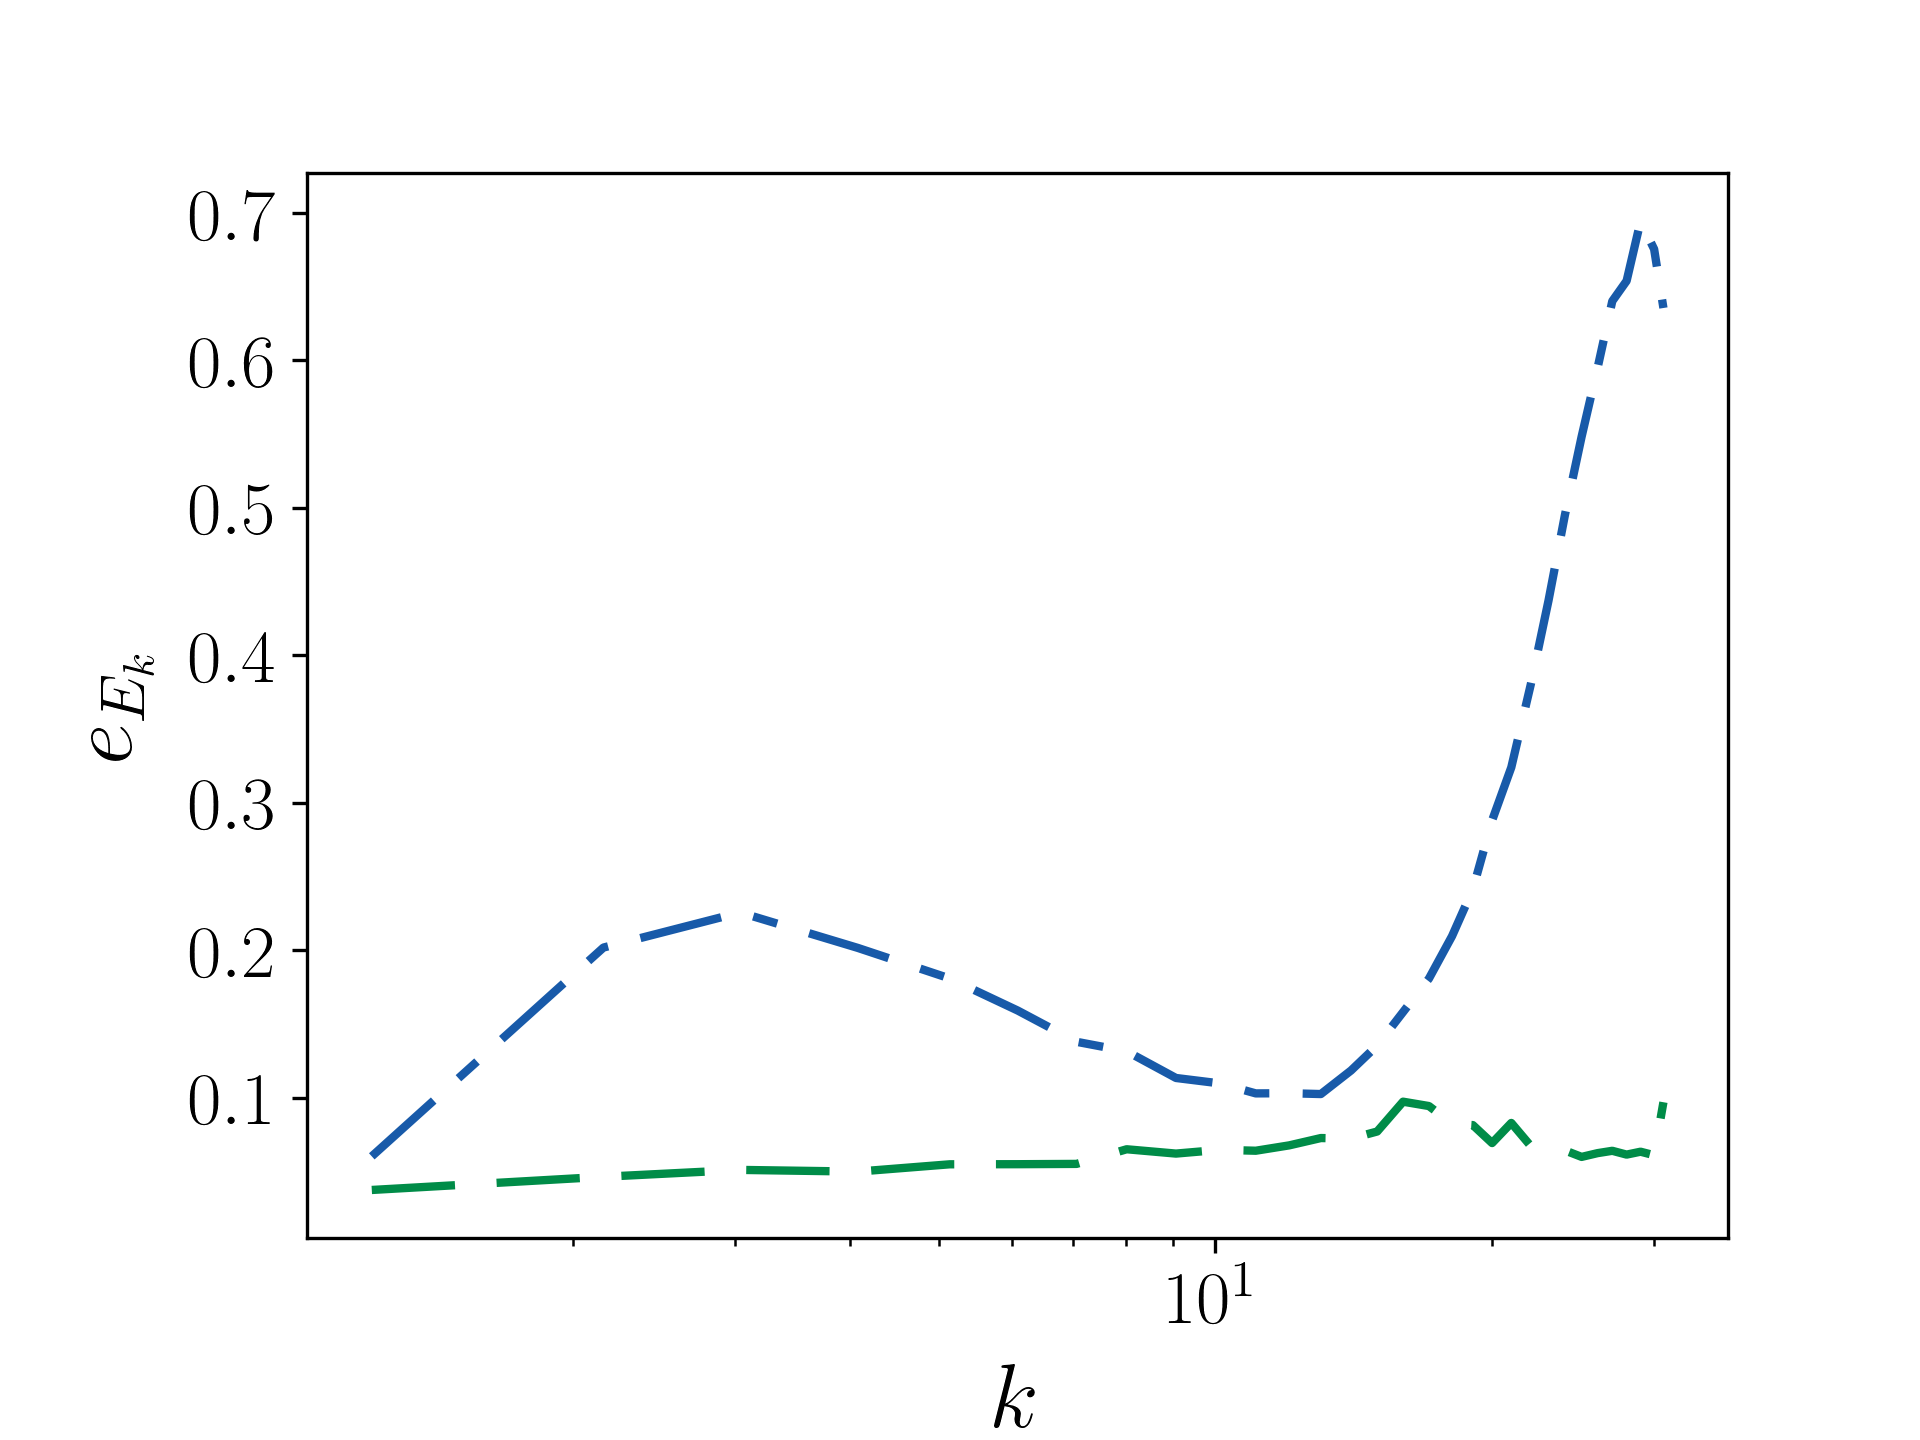
\includegraphics[width=\textwidth]{../../paper/figs/error_spectra.png}%
      \caption*{Normalized error, $e_{E_k} = \frac{|E^h_k - E_k|}{E_k}$.}\label{fig:error_spectra}%
    \end{subfigure}%
  \end{figure}%
  \structure{Results indicate that}\\
  \hspace*{1cm}CNN can represent the wide range of scales\\
  \hspace*{1cm}GPR under/overpredicts the intermediate/small scales
}

\frame{
  \frametitle{Recovered data is used in forward simulations of decay of homogeneous isotropic turbulence in PeleC.}
  \begin{figure}[!tbp]%
    \centering%
    Normalized enstrophy ($25\%$ of the original data is missing) 
    \begin{subfigure}[t]{0.48\textwidth}%
      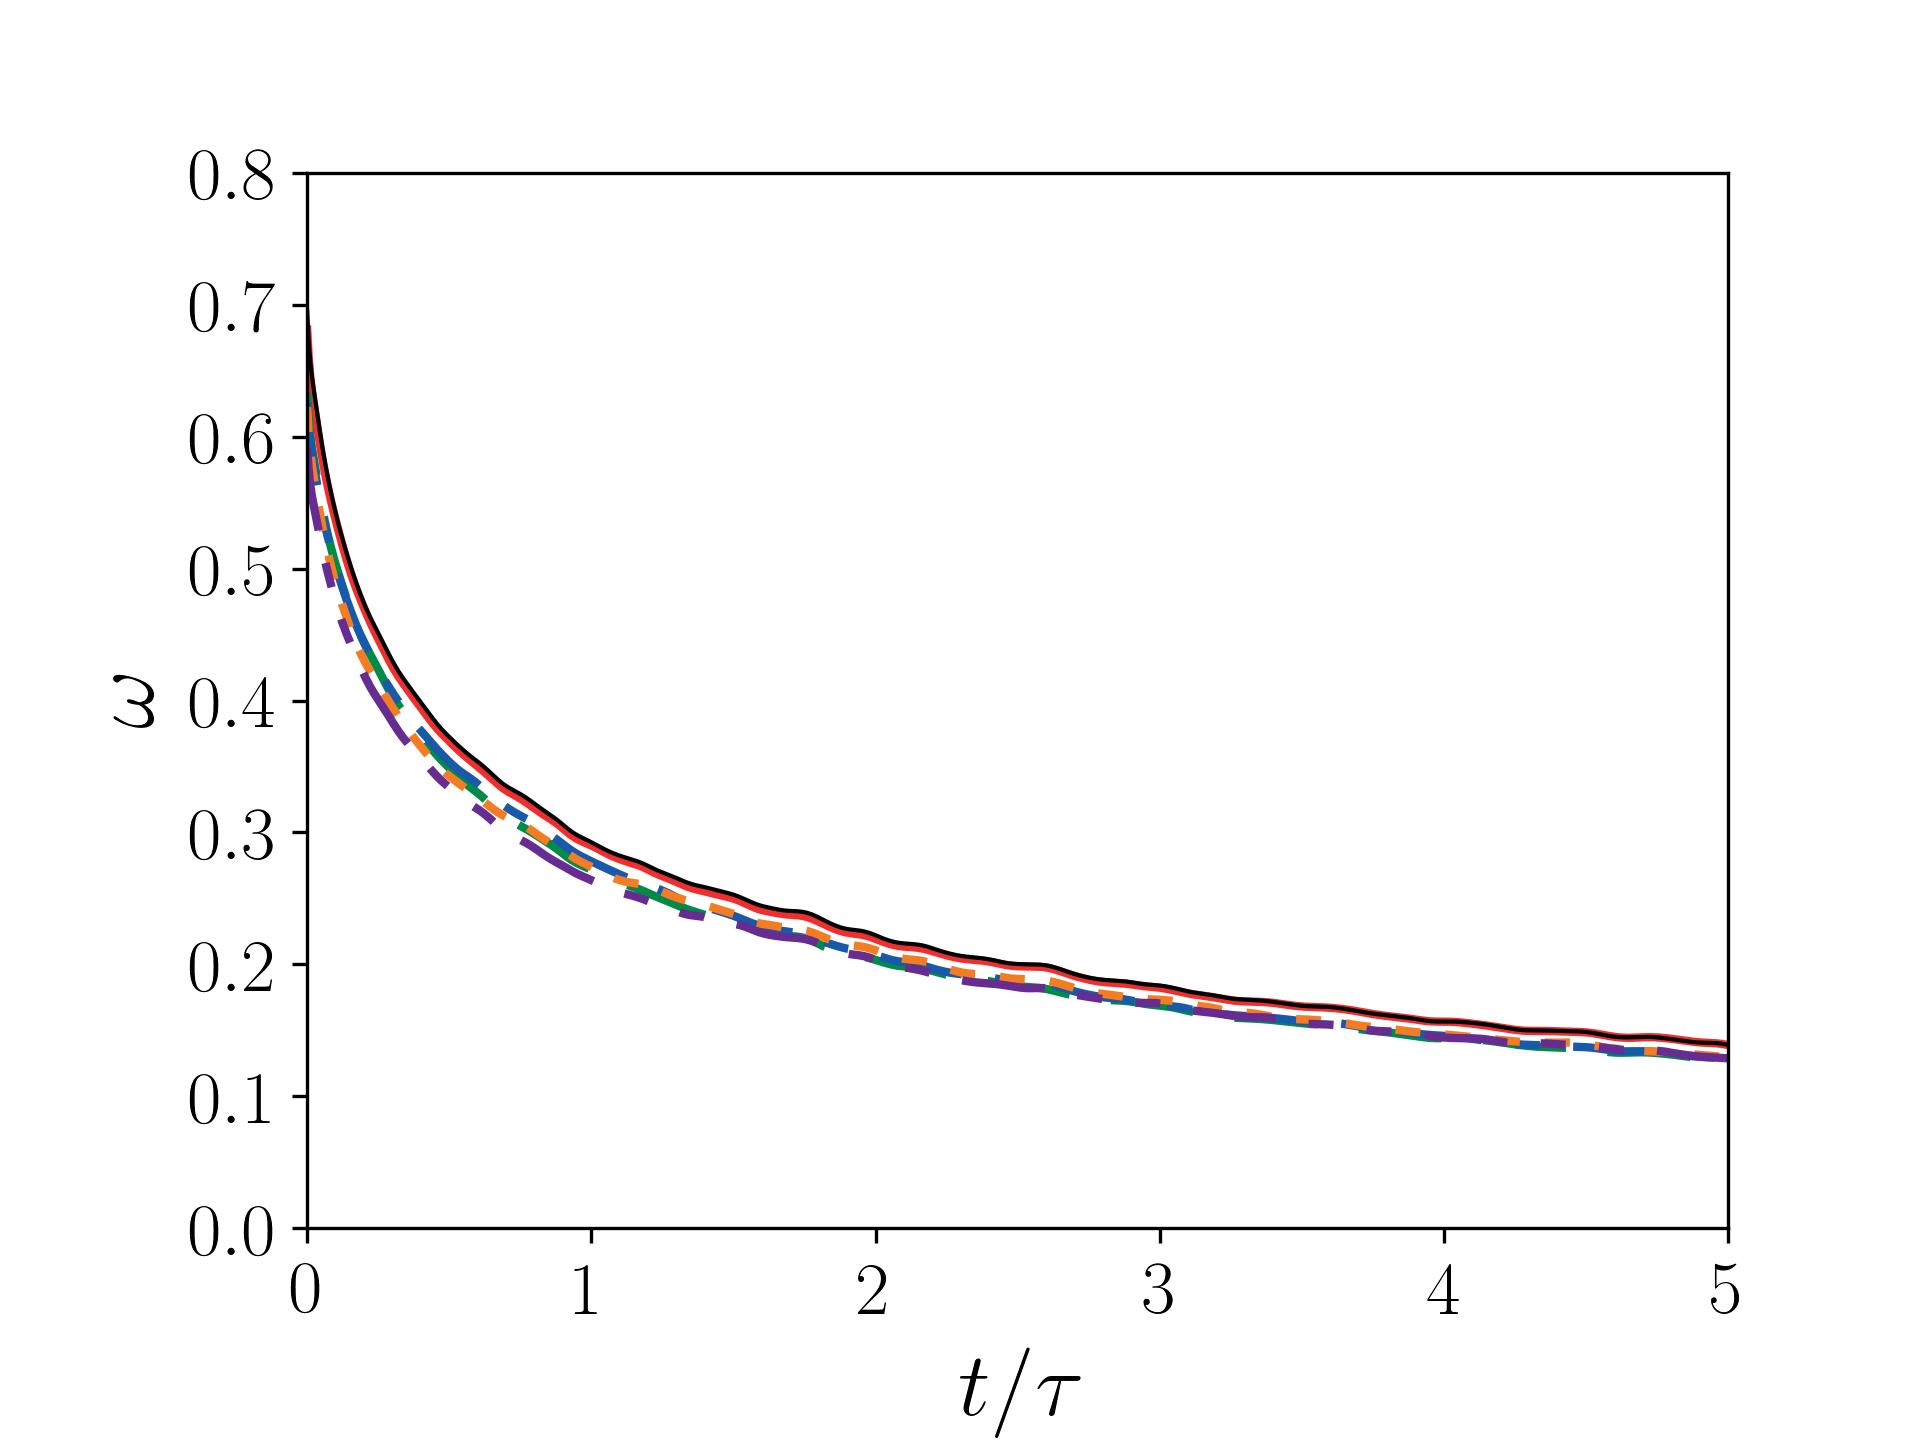
\includegraphics[width=\textwidth]{../../paper/figs/enstrophy_result.png}%
      \caption*{CNN.}\label{fig:enstrophy_dl}%
    \end{subfigure}%
    \hfill%
    \begin{subfigure}[t]{0.48\textwidth}%
      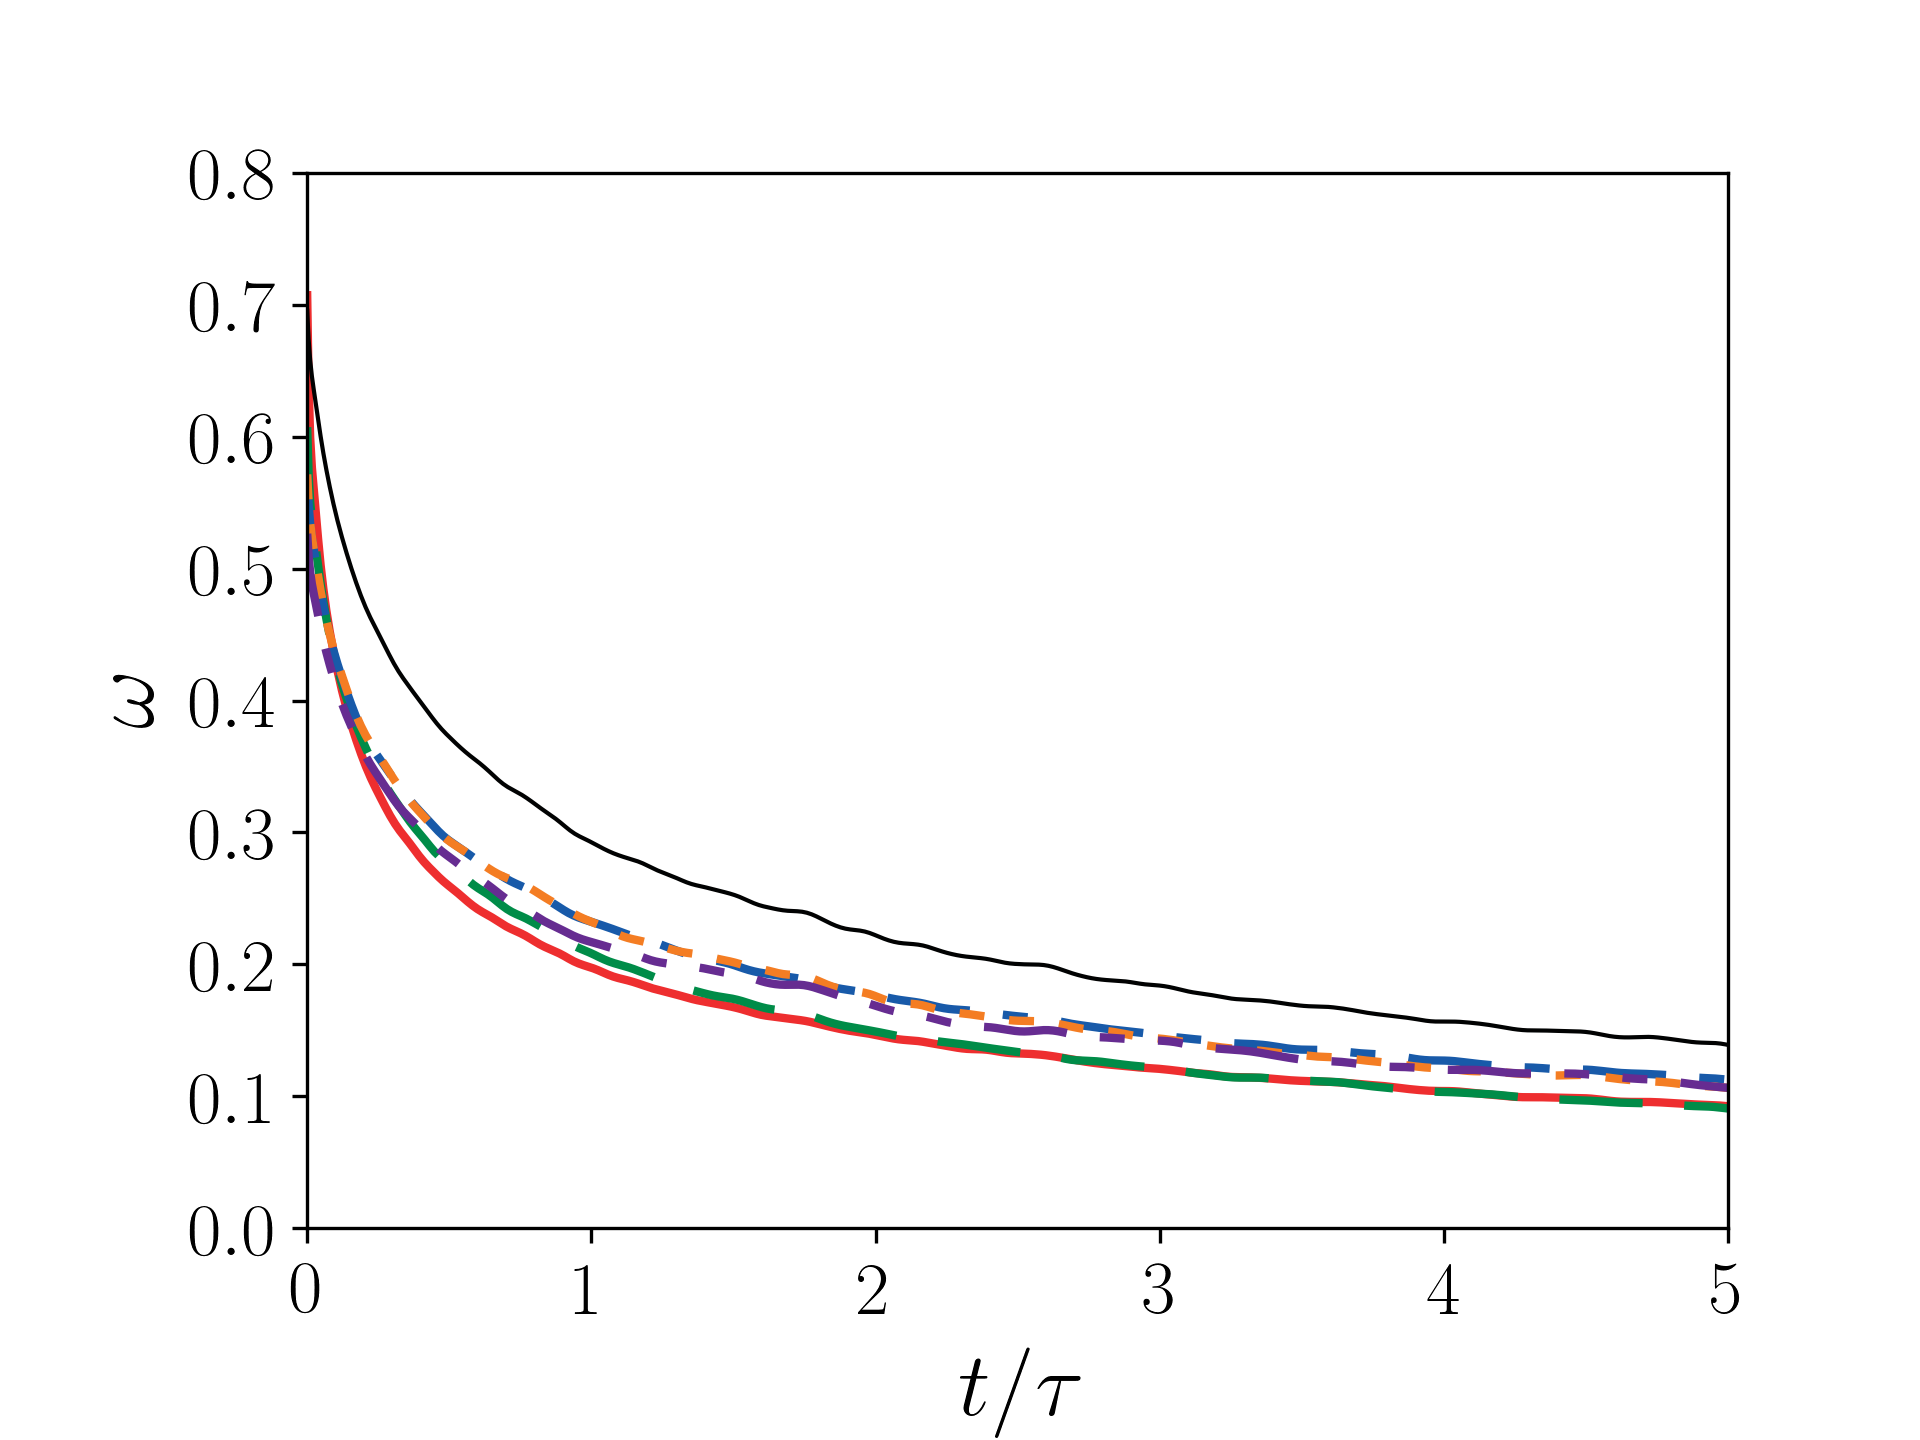
\includegraphics[width=\textwidth]{../../paper/figs/enstrophy_interp.png}%
      \caption*{GPR.}\label{fig:enstrophy_gp}%
    \end{subfigure}%
    \caption*{Solid black: original data;
      \textcolor{c1brt}{solid red:} $L_m=0.74\lambda$;
      \textcolor{c2brt}{dashed green}: $L_m=1.48\lambda$;
      \textcolor{c3brt}{dot-dashed blue}: $L_m=2.97\lambda$;
      \textcolor{c4brt}{dotted orange}: $L_m=5.94\lambda$;
      \textcolor{c5brt}{dot-dot-dashed purple}:
      $L_m=11.87\lambda$.}\label{fig:hit_enstrophy}%
  \end{figure}%
}

% ================================================================================
% Conclusions
\frame{
  \frametitle{We used deep convolutional neural networks for data recovery in computational fluid dynamics.}
  \structure{We demonstrated a method to recover the lost data that}\\
  \hspace*{1cm}is agnostic to the simulation configuration and geometry\\
  \hspace*{1cm}does not require extensive training data\\
  \hspace*{1cm}is accurate for very different physics\\[0.4cm]
  \structure{We successfully recovered data from different CFD flows}\\
  \hspace*{1cm}laminar flow around a cylinder (wake recovery)\\
  \hspace*{1cm}homogeneous isotropic turbulence (spectra recovery)\\[0.4cm]
  \structure{\mbox{Public repo: \url{https://github.com/NREL/deep-image-prior-cfd}}}\\
  \structure{Full paper: \url{http://arxiv.org/abs/1901.11113}}\\[0.4cm]
  {\tiny\textit{This research was supported by the Exascale Computing Project (ECP), Project Number: 17-SC-20-SC, a collaborative effort of two DOE organizations -- the Office of Science and the National Nuclear Security Administration -- responsible for the planning and preparation of a capable exascale ecosystem -- including software, applications, hardware, advanced system engineering, and early testbed platforms -- to support the nation's exascale computing imperative.}\par}
}

% =================================================================================
% Bibliography
\begin{frame}[allowframebreaks,plain]{Bibliography}
  \tiny
  \bibliographystyle{model1-num-names}
  %\bibliographystyle{jap}
  \bibliography{../../paper/library}
\end{frame}

\egroup

\end{document}
